%%%%%%%%%%%%%%%%%%%%%%%%%%%%%%%%%%%%%%%%%
% The Legrand Orange Book
% LaTeX Template - adaptado
%
% Memoria Estancia en Prácticas - IR2137
% Mario García Blasco
% V4R Lab, ACIN, TU Wien
%
% Compilación:
% 1) pdflatex main
% 2) makeindex main.idx -s StyleInd.ist
% 3) biber main
% 4) pdflatex main x 2
%%%%%%%%%%%%%%%%%%%%%%%%%%%%%%%%%%%%%%%%%


%----------------------------------------------------------------------------------------
%	PACKAGES AND OTHER DOCUMENT CONFIGURATIONS
%----------------------------------------------------------------------------------------

\documentclass[11pt,fleqn,openany]{book} % openany evita páginas en blanco antes de cada chapter

\input{structure} % Insert the commands.tex file


% ---------------------------------------------------------------------
%  Paquetes y librerías adicionales (no se modifica el bloque del Gantt)
% ---------------------------------------------------------------------
\usepackage{tikz,times}
\usepackage{verbatim}
\usepackage{graphicx}
\usepackage{pdflscape}
\usepackage[font=small,labelfont={bf,color=ocre},labelsep=colon,
            justification=centering,singlelinecheck=true]{caption}
\usepackage{colortbl}    % for row coloring in tables

% Make \cite produce parenthetical citations like (Author, year) by default,
% which reads better inline in Spanish technical prose.
\let\cite=\parencite

% Use "Tabla" instead of the babel-spanish default "Cuadro" for table captions.
% More natural in modern technical Spanish, especially in engineering.
\addto\captionsspanish{\renewcommand{\tablename}{Tabla}\renewcommand{\listtablename}{LISTA DE TABLAS}}

% Aggressive widow / orphan control to avoid lonely lines at page breaks.
\widowpenalty=10000
\clubpenalty=10000
\displaywidowpenalty=10000
\raggedbottom

% Highlighted subtitle command for the course-level groupings in Cap 4.
% Gives the "Primer curso" / "Segundo curso" / etc. headings a clear visual
% break above and a coloured rule below, distinguishing them from the
% \paragraph{} subject names that follow.
\newcommand{\cursoTitulo}[1]{%
  \par\addvspace{14pt}%
  {\sffamily\bfseries\large\color{ocre}#1}%
  \par\vspace{1pt}%
  \noindent{\color{ocre!60}\rule{\linewidth}{0.4pt}}%
  \par\addvspace{4pt}%
}

% Override the template's "figure" entry style for the Lista de Figuras so
% that consecutive figure entries don't collide (the original template uses
% \addvspace{-5pt} which makes lines overlap).
\titlecontents{figure}[1.5em]
  {\addvspace{4pt}\sffamily\small}
  {\contentslabel[\thecontentslabel]{1.8em}}
  {}
  {\ \titlerule*[.5pc]{.}\;\thecontentspage}
  []
\titlecontents{table}[1.5em]
  {\addvspace{4pt}\sffamily\small}
  {\contentslabel[\thecontentslabel]{1.8em}}
  {}
  {\ \titlerule*[.5pc]{.}\;\thecontentspage}
  []
\usetikzlibrary{positioning}
\usetikzlibrary{arrows.meta}
\usetikzlibrary{shapes.geometric}
\usetikzlibrary{shapes.misc}
\usetikzlibrary{fit}
\usetikzlibrary{calc}
\usetikzlibrary{backgrounds}
\usetikzlibrary{shadows}
\usetikzlibrary{decorations.pathmorphing}
\usetikzlibrary{mindmap,trees}

% Colores antiguos del template (no se eliminan)
\definecolor{color_mate}{RGB}{255,255,128}
\definecolor{color_petr}{RGB}{255,192,192}
\definecolor{color_made}{RGB}{192,255,192}
\definecolor{color_meta}{RGB}{192,192,255}
\definecolor{color_text}{RGB}{255,150,150}
\definecolor{color_plas}{RGB}{150,150,255}

% Paleta propia para las figuras explicativas
\definecolor{figAzul}{RGB}{222,238,250}
\definecolor{figAzulBorde}{RGB}{60,120,180}
\definecolor{figVerde}{RGB}{225,242,225}
\definecolor{figVerdeBorde}{RGB}{60,135,80}
\definecolor{figNaranja}{RGB}{252,232,200}
\definecolor{figNaranjaBorde}{RGB}{200,120,40}
\definecolor{figVioleta}{RGB}{235,225,245}
\definecolor{figVioletaBorde}{RGB}{120,80,160}
\definecolor{figGris}{RGB}{240,240,240}
\definecolor{figGrisBorde}{RGB}{120,120,120}

% Estilos comunes para las figuras
\tikzset{
  bloque/.style={
    rectangle, rounded corners=4pt, draw=figAzulBorde, line width=0.7pt,
    fill=figAzul, minimum height=0.95cm, minimum width=2.6cm,
    align=center, font=\sffamily\small, inner sep=4pt
  },
  bloquev/.style={
    rectangle, rounded corners=4pt, draw=figVerdeBorde, line width=0.7pt,
    fill=figVerde, minimum height=0.95cm, minimum width=2.6cm,
    align=center, font=\sffamily\small, inner sep=4pt
  },
  bloquen/.style={
    rectangle, rounded corners=4pt, draw=figNaranjaBorde, line width=0.7pt,
    fill=figNaranja, minimum height=0.95cm, minimum width=2.6cm,
    align=center, font=\sffamily\small, inner sep=4pt
  },
  bloquei/.style={
    rectangle, rounded corners=4pt, draw=figVioletaBorde, line width=0.7pt,
    fill=figVioleta, minimum height=0.95cm, minimum width=2.6cm,
    align=center, font=\sffamily\small, inner sep=4pt
  },
  bloqueg/.style={
    rectangle, rounded corners=2pt, draw=figGrisBorde, line width=0.5pt,
    fill=figGris, minimum height=0.7cm, minimum width=2.2cm,
    align=center, font=\sffamily\footnotesize, inner sep=3pt
  },
  flecha/.style={-Latex, line width=0.8pt, draw=figAzulBorde!85!black},
  flechan/.style={-Latex, line width=0.8pt, draw=figNaranjaBorde!85!black, dashed},
  grupo/.style={
    rounded corners=6pt, draw=figGrisBorde, line width=0.5pt, dashed,
    inner sep=8pt
  }
}


\begin{document}

%----------------------------------------------------------------------------------------
%	TITLE PAGE
%----------------------------------------------------------------------------------------

\begingroup
\thispagestyle{empty}
\begin{tikzpicture}[remember picture,overlay]
\node[inner sep=0pt] (background) at (current page.center) {
\includegraphics[width=\paperwidth]{background}};
\draw (current page.center) node [fill=ocre!30!white,fill opacity=0.6,text opacity=1,inner sep=1cm]{\Huge\centering\bfseries\sffamily\parbox[c][][t]{\paperwidth}{\centering MEMORIA ESTANCIA EN PRÁCTICAS\\[15pt] % Book title
{\huge Grado Inteligencia Robótica\\Universidad Jaume I de Castellón}\\[12pt] % Subtitle
{\huge Búsqueda Semántica de Objetos en Simulación
con Razonamiento por Habitaciones}\\[14pt] % Subtitle
{\Large Estudiante: Mario García Blasco
 \\Tutor: Alejandro Reig Gisbert
 \\Supervisores: Markus Vincze y Tessa Pulli}}}; % Author name

\end{tikzpicture}
\vfill
\endgroup

%----------------------------------------------------------------------------------------
%	TABLE OF CONTENTS
%----------------------------------------------------------------------------------------

\usechapterimagefalse

\pagestyle{empty}

\renewcommand{\contentsname}{TABLA DE CONTENIDOS}
\tableofcontents

\clearpage

\pagestyle{fancy}


%----------------------------------------------------------------------------------------
%	CAPÍTULO 1: INTRODUCCIÓN
%----------------------------------------------------------------------------------------

\chapter{Introducción}

\section{Resumen}

Esta memoria documenta las 150 horas correspondientes a la asignatura IR2137, Prácticas Externas, del Grado en Inteligencia Robótica de la Universitat Jaume I. La estancia se realizó en el Vision for Robotics Group (V4R) del Automation and Control Institute (ACIN) de la Technische Universität Wien, bajo la supervisión de Tessa Pulli y Markus Vincze, y con el seguimiento académico de Alejandro Reig Gisbert.

El proyecto aborda la búsqueda semántica de objetos en entornos interiores simulados a partir de instrucciones en lenguaje natural. El problema no se plantea como una simple navegación hacia el punto con mayor activación semántica, sino como una decisión estructurada: el robot debe decidir primero en qué habitación tiene sentido buscar, después qué zona o mueble inspeccionar y, finalmente, confirmar visualmente si el objeto está presente. La aportación principal de las prácticas es estudiar la viabilidad de construir, sobre la memoria semántica proporcionada por VLMaps, una arquitectura de búsqueda jerárquica que combina selección de habitación, consulta de zonas candidatas, navegación y verificación visual con YOLOE.

La memoria recoge, en el cuerpo principal, las tres primeras quincenas de trabajo, que constituyen el alcance real de las prácticas. La cuarta quincena se presenta de forma diferenciada, en un capítulo dedicado a la continuidad del proyecto dentro del Trabajo de Final de Grado.

\medskip
\noindent\textbf{Palabras clave:} búsqueda semántica de objetos, razonamiento por habitaciones, simulación robótica, visión por computador, modelos de visión-lenguaje, ROS.

\section{Datos identificativos}

Soy Mario García Blasco, estudiante del Grado en Inteligencia Robótica en la Universitat Jaume I de Castellón. Durante el periodo de Prácticas Externas he realizado mi estancia en el Vision for Robotics Group (V4R), perteneciente al Automation and Control Institute (ACIN) de la Technische Universität Wien, en Viena. He contado con la supervisión conjunta de Tessa Pulli, investigadora doctoral, y de Markus Vincze, que además dirige el grupo de investigación. El seguimiento académico ha estado a cargo de Alejandro Reig Gisbert.

La estancia completa está prevista entre el 1 de marzo y el 30 de mayo de 2026. Esta memoria recoge únicamente el trabajo correspondiente a las 150 horas asociadas a la asignatura IR2137, Prácticas Externas. Con una dedicación aproximada de cinco horas diarias, esas horas equivalen a unas seis semanas efectivas de trabajo. Por este motivo, el cuerpo principal se centra en las tres primeras quincenas, desde el inicio de marzo hasta el 20 de abril de 2026. Las actividades posteriores se separan en el capítulo \emph{Continuación de Tareas en el TFG}, para distinguir con claridad lo desarrollado dentro de las prácticas de lo que se proyecta para el Trabajo de Final de Grado.

El proyecto se centra en la búsqueda semántica de objetos en entornos interiores simulados. En términos prácticos, el objetivo es que un robot pueda recibir órdenes como \emph{encuentra el portátil}, \emph{busca la botella} o \emph{ve a la cocina y comprueba si hay una taza}, interpretar la petición, decidir dónde tiene sentido buscar y desplazarse hasta una zona candidata para verificar visualmente el objeto. La dificultad está en evitar una búsqueda plana sobre el mapa semántico: para un objeto doméstico, no basta con elegir el punto de mayor puntuación; también hay que razonar sobre habitaciones, muebles y visibilidad. La figura~\ref{fig:toyota_hsr_intro} muestra el tipo de robot doméstico de servicio que se considera como plataforma futura para esta línea de trabajo.

\begin{figure}[H]
\centering

\includegraphics[width=0.82\linewidth]{toyota-human-support-robot-2.png}
\caption[Toyota Human Support Robot.]{Toyota Human Support Robot (HSR), plataforma móvil doméstica de referencia para la integración futura del sistema.\protect\footnotemark}
\label{fig:toyota_hsr_intro}
\end{figure}
\footnotetext{Imagen tomada de la sala de prensa oficial de Toyota Motor Europe: \href{https://media.toyota.co.uk/toyota-accelerates-home-helper-robot-programme-with-new-developer-community-and-working-prototype/}{media.toyota.co.uk} (acceso: mayo de 2026).}

\section{Descripción del centro/empresa}

El V4R Lab forma parte del Automation and Control Institute (ACIN) de la Technische Universität Wien. Se trata de un entorno universitario y de investigación dedicado al desarrollo de soluciones en percepción robótica, comprensión semántica de escenas, manipulación de objetos e interacción humano-robot. La actividad del grupo combina visión por computador, sensores RGB-D, planificación de movimiento y sistemas inteligentes de percepción, con un enfoque claramente aplicado dentro de la investigación universitaria.

Durante los primeros días en el laboratorio, Tessa Pulli, Markus Vincze y el grupo de investigación me presentaron distintas posibilidades de trabajo dentro de la navegación semántica. Una de las opciones iniciales consistía en utilizar VLMaps para mapear un entorno de oficina y estudiar su utilidad como representación semántica. A partir de esa propuesta, el objetivo de las prácticas no fue limitarse a generar o consultar un mapa semántico, sino estudiar si esa representación podía servir como memoria semántica para una arquitectura de búsqueda de objetos más completa. En ella, la selección de habitación decide dónde buscar, el mapa propone zonas o muebles candidatos y YOLOE verifica visualmente si el objeto concreto está presente.

\begin{figure}[H]
\centering
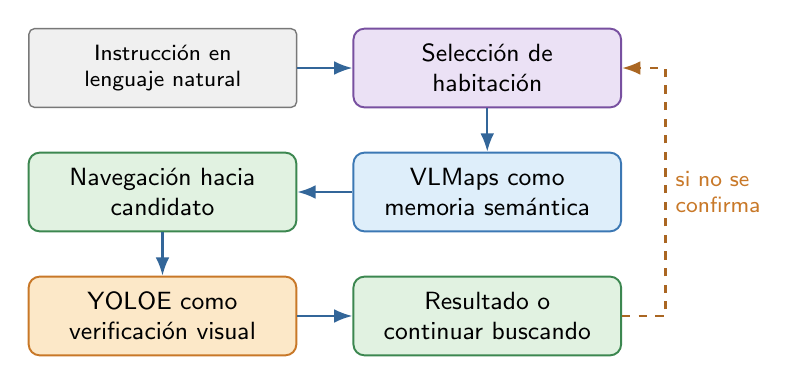
\begin{tikzpicture}[node distance=0.55cm and 0.7cm]
  \node[bloqueg, minimum width=3.4cm, minimum height=1.0cm] (instr)
    {Instrucción en\\lenguaje natural};
  \node[bloquei, minimum width=3.4cm, minimum height=1.0cm, right=of instr] (sel)
    {Selección de\\habitación};
  \node[bloque, minimum width=3.4cm, minimum height=1.0cm, below=of sel] (vlmaps)
    {VLMaps como\\memoria semántica};
  \node[bloquev, minimum width=3.4cm, minimum height=1.0cm, left=of vlmaps] (nav)
    {Navegación hacia\\candidato};
  \node[bloquen, minimum width=3.4cm, minimum height=1.0cm, below=of nav] (yoloe)
    {YOLOE como\\verificación visual};
  \node[bloquev, minimum width=3.4cm, minimum height=1.0cm, right=of yoloe] (res)
    {Resultado o\\continuar buscando};

  \draw[flecha] (instr) -- (sel);
  \draw[flecha] (sel) -- (vlmaps);
  \draw[flecha] (vlmaps) -- (nav);
  \draw[flecha] (nav) -- (yoloe);
  \draw[flecha] (yoloe) -- (res);

  \draw[flechan] (res.east) -- ++(0.55,0) |- (sel.east)
        node[pos=0.25, right, font=\sffamily\footnotesize, text=figNaranjaBorde, align=left]
        {si no se\\confirma};
\end{tikzpicture}
\caption[Idea general del enfoque propuesto.]{Idea general del enfoque: el mapa semántico actúa como memoria sobre la que se selecciona habitación, candidato y, tras la navegación, se verifica con YOLOE.}
\label{fig:arquitectura_general}
\end{figure}

Durante la estancia he tenido acceso a un puesto de trabajo con los recursos de cómputo necesarios, soporte por parte del equipo y reuniones periódicas para discutir el avance del proyecto. La supervisión combinó orientación técnica, validación de decisiones y autonomía progresiva. Las actividades realizadas se alinean con las tareas previstas en la propuesta de prácticas: análisis técnico de segmentación semántica y planificación, integración de programas y sensores, implementación de algoritmos de comprensión de escena, realización de pruebas experimentales y documentación de la metodología y de los resultados.

\section{Agradecimientos}

Quiero expresar mi agradecimiento a Tessa Pulli y a Markus Vincze, supervisores directos de la estancia en el V4R Lab, por su orientación, su disponibilidad y la calidad de las conversaciones técnicas que han permitido enmarcar correctamente el alcance del proyecto. Markus, además de supervisor, dirige el grupo de investigación y aportó el marco general en el que se ha desarrollado el trabajo.

Al tutor académico Alejandro Reig Gisbert, por el acompañamiento desde la Universitat Jaume I y por asegurar que la planificación de las prácticas se ajustaba a los requisitos de la asignatura IR2137.

De forma especial, quiero agradecer a Pau Montagut Bofi haberse lanzado conmigo a esta aventura. Ha sido la persona con la que más codo a codo he trabajado durante la estancia, y compartir con él tanto las dificultades técnicas como el día a día en Viena ha hecho que el periodo de prácticas tenga mucho más valor.

Y, en general, al resto de personas del Vision for Robotics Group que han hecho de la estancia una experiencia profesional y personal especialmente valiosa.

\medskip

\subsection*{Glosario rápido}

Para que los siguientes capítulos resulten cómodos de leer, se recogen aquí los términos que más se repiten.

\begin{description}[leftmargin=2.2em,style=nextline,itemsep=2pt]
  \item[VLMaps] Representación que asocia cada celda de un mapa 2D con categorías visuales generales (mesa, sofá, encimera, cama, etc.), usando modelos de visión-lenguaje. En este proyecto actúa como memoria semántica del entorno.
  \item[YOLOE] Detector visual de vocabulario abierto. Recibe una etiqueta textual y comprueba en la imagen de la cámara si el objeto está presente. Cierra la cadena de búsqueda como verificador final.
  \item[Mapa de calor semántico] Salida 2D del mapa semántico para una categoría: cada celda lleva una puntuación de afinidad con esa categoría. Es el insumo del que se extraen las zonas candidatas.
  \item[Habitat-Sim] Simulador 3D usado para mover un robot virtual por escenas interiores y probar el flujo completo sin hardware.
  \item[HSSD / Matterport3D] Conjuntos de escenas interiores. HSSD se usa como entorno principal porque incluye anotaciones nativas de habitaciones; Matterport3D queda como soporte secundario.
  \item[CLIP / LSeg] Modelos de visión-lenguaje sobre los que se apoya el mapa semántico para asociar regiones del entorno con categorías generales.
  \item[Razonamiento por habitaciones] Estrategia de búsqueda jerárquica en tres niveles: habitación, zona o mueble y objeto concreto.
  \item[Ejecutor estructurado] Variante del sistema que organiza la búsqueda como una secuencia explícita de acciones de alto nivel (ir a una habitación, explorar, inspeccionar un candidato, verificar el objeto, terminar).
  \item[ROS, Gazebo, RViz] Herramientas estándar en robótica para navegación, simulación y visualización. Se utilizan en el contenedor de navegación robótica.
  \item[rosbridge] Puente que permite comunicar el contenedor semántico con el contenedor de ROS mediante WebSocket.
  \item[Toyota HSR] Robot móvil doméstico de servicio que se toma como plataforma de referencia para la integración futura.
\end{description}

\subsection*{Estructura de la memoria}

Para facilitar la lectura, este documento se organiza en seis capítulos numerados y una bibliografía final. El capítulo~\ref{chap:actividades} describe las actividades realizadas, organizadas en bloques temáticos coherentes con el diagrama de Gantt. El capítulo~\ref{chap:resultados} resume los resultados obtenidos, los recursos utilizados y el apoyo recibido durante la estancia. El capítulo~\ref{chap:tfg} plantea las líneas de continuidad dentro del Trabajo de Final de Grado, separadas del periodo principal de prácticas. El capítulo~\ref{chap:competencias} relaciona el trabajo con asignaturas concretas del Grado en Inteligencia Robótica de la Universitat Jaume I. El capítulo~\ref{chap:conclusion} cierra la memoria con una valoración técnica y personal.

%----------------------------------------------------------------------------------------
%	CAPÍTULO 2: ACTIVIDADES REALIZADAS
%----------------------------------------------------------------------------------------

\chapter{Actividades Realizadas}\label{chap:actividades}

\section{Diagrama de Gantt}

Con el fin de contextualizar el desarrollo de las prácticas, la figura~\ref{fig:gantt} presenta una planificación por semanas efectivas de trabajo. La semana correspondiente a las vacaciones de Pascua no se incluye en el eje temporal, ya que durante ese periodo no se computaron horas de prácticas. Las tareas 1 a 9 suman las 150 horas correspondientes a la asignatura IR2137, mientras que las tareas posteriores recogen la continuación del trabajo dentro del TFG.

% Paleta azul del diagrama original
\definecolor{ganttFondo}{RGB}{237,249,251}
\definecolor{ganttTrabajo}{RGB}{186,231,240}
\definecolor{ganttTrabajoTFG}{RGB}{126,210,226}
\definecolor{ganttLinea}{RGB}{0,145,170}
\definecolor{ganttFase}{RGB}{0,150,180}
\definecolor{ganttCabecera}{RGB}{222,246,250}
\definecolor{ganttTexto}{RGB}{35,35,35}
\definecolor{ganttGuia}{RGB}{210,240,246}

\begin{landscape}
\thispagestyle{plain}

\begin{center}
\vspace*{-0.75cm}

\resizebox{0.985\linewidth}{!}{%
\begin{tikzpicture}[
    x=2.05cm,
    y=0.83cm,
    font=\sffamily,
    tasklabel/.style={
        align=left,
        text width=6.85cm,
        font=\normalsize,
        text=ganttTexto,
        inner sep=2pt
    },
    weeklabel/.style={
        align=center,
        font=\bfseries\normalsize,
        text=ganttTexto
    },
    phaselabel/.style={
        align=center,
        font=\bfseries\normalsize,
        text=white,
        text width=4.05cm,
        inner sep=2pt,
        execute at begin node=\setlength{\baselineskip}{12pt}
    },
    bartext/.style={
        font=\bfseries\small,
        text=ganttTexto
    }
]

% =====================================================================
% Parámetros
% =====================================================================
\def\ntasks{15}
\def\nweeks{8}
\def\taskwidth{3.55}
\def\headerA{15.00}
\def\headerB{15.95}
\def\headerC{17.45}

% =====================================================================
% Fondo general
% =====================================================================
\fill[ganttFondo] (-\taskwidth,0) rectangle (\nweeks,\headerC);

% Bandas alternas para leer mejor las filas
\foreach \y in {0,2,4,6,8,10,12,14} {
    \fill[ganttCabecera, opacity=0.35]
        (-\taskwidth,\y) rectangle (\nweeks,\y+1);
}

% =====================================================================
% Cuadrícula
% =====================================================================

% Subdivisiones diarias, 5 días por semana
\foreach \d in {1,...,39} {
    \pgfmathsetmacro{\x}{\d/5}
    \draw[ganttGuia, line width=0.16pt, opacity=0.22]
        (\x,0) -- (\x,\ntasks);
}

% Separadores de semana
\foreach \w in {1,...,7} {
    \draw[ganttLinea, line width=0.75pt]
        (\w,0) -- (\w,\headerB);
}

% Separadores de filas
\foreach \y in {1,...,14} {
    \draw[ganttGuia, line width=0.20pt, opacity=0.55]
        (-\taskwidth,\y) -- (\nweeks,\y);
}

% División entre tareas y calendario
\draw[ganttLinea, line width=1.05pt]
    (0,0) -- (0,\headerC);

% =====================================================================
% Cabecera de semanas
% =====================================================================
\foreach \w in {0,...,7} {
    \pgfmathtruncatemacro{\num}{\w+1}
    \draw[ganttLinea, fill=ganttCabecera, line width=0.55pt]
        (\w,\headerA) rectangle (\w+1,\headerB);
    \node[weeklabel] at (\w+0.5,{(\headerA+\headerB)/2})
        {Semana \num};
}

% =====================================================================
% Cabecera de fases
% =====================================================================
\draw[ganttLinea, fill=ganttFase, line width=0.60pt]
    (0,\headerB) rectangle (2,\headerC);
\node[phaselabel] at (1,{(\headerB+\headerC)/2})
    {Preparación\\inicial};

\draw[ganttLinea, fill=ganttFase, line width=0.60pt]
    (2,\headerB) rectangle (4,\headerC);
\node[phaselabel] at (3,{(\headerB+\headerC)/2})
    {Navegación\\y percepción};

\draw[ganttLinea, fill=ganttFase, line width=0.60pt]
    (4,\headerB) rectangle (6,\headerC);
\node[phaselabel] at (5,{(\headerB+\headerC)/2})
    {Razonamiento\\por habitaciones};

\draw[ganttLinea, fill=ganttFase, line width=0.60pt]
    (6,\headerB) rectangle (8,\headerC);
\node[phaselabel] at (7,{(\headerB+\headerC)/2})
    {Continuación\\del TFG};

% =====================================================================
% Cabecera de tareas
% =====================================================================
\draw[ganttLinea, fill=ganttFase, line width=0.70pt]
    (-\taskwidth,\headerA) rectangle (0,\headerC);

\node[font=\bfseries\LARGE, text=white]
    at ({-\taskwidth/2},{(\headerA+\headerC)/2})
    {Tareas};

% =====================================================================
% Etiquetas de tareas
% =====================================================================
\node[tasklabel, anchor=west] at ({-\taskwidth+0.08},14.5)
    {\textbf{1.} Preparación del entorno};

\node[tasklabel, anchor=west] at ({-\taskwidth+0.08},13.5)
    {\textbf{2.} Configuración de Docker y CUDA};

\node[tasklabel, anchor=west] at ({-\taskwidth+0.08},12.5)
    {\textbf{3.} Integración de Habitat-Sim};

\node[tasklabel, anchor=west] at ({-\taskwidth+0.08},11.5)
    {\textbf{4.} Integración de VLMaps};

\node[tasklabel, anchor=west] at ({-\taskwidth+0.08},10.5)
    {\textbf{5.} Navegación inicial};

\node[tasklabel, anchor=west] at ({-\taskwidth+0.08},9.5)
    {\textbf{6.} Integración de YOLOE};

\node[tasklabel, anchor=west] at ({-\taskwidth+0.08},8.5)
    {\textbf{7.} Filtros y calidad de candidatos};

\node[tasklabel, anchor=west] at ({-\taskwidth+0.08},7.5)
    {\textbf{8.} Razonamiento por habitaciones};

\node[tasklabel, anchor=west] at ({-\taskwidth+0.08},6.5)
    {\textbf{9.} Estado estructurado de búsqueda};

\node[tasklabel, anchor=west] at ({-\taskwidth+0.08},5.5)
    {\textbf{10.} Evaluación del mapa de calor};

\node[tasklabel, anchor=west] at ({-\taskwidth+0.08},4.5)
    {\textbf{11.} Comparación de orquestadores};

\node[tasklabel, anchor=west] at ({-\taskwidth+0.08},3.5)
    {\textbf{12.} Preparación del entorno ROS};

\node[tasklabel, anchor=west] at ({-\taskwidth+0.08},2.5)
    {\textbf{13.} Puesta en marcha de Gazebo y RViz};

\node[tasklabel, anchor=west] at ({-\taskwidth+0.08},1.5)
    {\textbf{14.} Integración con ROS 1 Noetic y HSR};

\node[tasklabel, anchor=west] at ({-\taskwidth+0.08},0.5)
    {\textbf{15.} Validación de la migración};

% =====================================================================
% Barras de tareas
% Coordenadas en semanas. Cada 0.2 equivale a un día útil.
% =====================================================================
\def\barraGanttMario#1#2#3#4#5{%
    % Anchura mínima visual para que las barras cortas no aplasten el texto
    \pgfmathsetmacro{\barcenter}{(#1+#2)/2}
    \pgfmathsetmacro{\barwidth}{#2-#1}
    \pgfmathsetmacro{\minbarwidth}{0.30}
    \pgfmathsetmacro{\drawwidth}{max(\barwidth,\minbarwidth)}
    \pgfmathsetmacro{\drawleft}{\barcenter-\drawwidth/2}
    \pgfmathsetmacro{\drawright}{\barcenter+\drawwidth/2}

    \path[
        fill=#5,
        draw=ganttLinea,
        line width=0.55pt,
        rounded corners=1.5pt
    ]
        (\drawleft,#3-0.39) rectangle (\drawright,#3+0.39);

    \node[bartext] at (\barcenter,#3) {#4};
}

% Prácticas: 150 h
\barraGanttMario{0.0}{0.6}{14.5}{15\,h}{ganttTrabajo}
\barraGanttMario{0.6}{1.0}{13.5}{10\,h}{ganttTrabajo}
\barraGanttMario{1.0}{1.6}{12.5}{15\,h}{ganttTrabajo}
\barraGanttMario{1.6}{2.0}{11.5}{10\,h}{ganttTrabajo}
\barraGanttMario{2.0}{2.4}{10.5}{10\,h}{ganttTrabajo}
\barraGanttMario{2.4}{3.4}{9.5}{25\,h}{ganttTrabajo}
\barraGanttMario{3.4}{4.2}{8.5}{20\,h}{ganttTrabajo}
\barraGanttMario{4.2}{5.4}{7.5}{30\,h}{ganttTrabajo}
\barraGanttMario{5.4}{6.0}{6.5}{15\,h}{ganttTrabajo}

% Continuación del TFG
\barraGanttMario{6.0}{6.2}{5.5}{5\,h}{ganttTrabajoTFG}
\barraGanttMario{6.2}{6.6}{4.5}{10\,h}{ganttTrabajoTFG}
\barraGanttMario{6.4}{6.8}{3.5}{10\,h}{ganttTrabajoTFG}
\barraGanttMario{6.8}{7.2}{2.5}{10\,h}{ganttTrabajoTFG}
\barraGanttMario{7.0}{7.6}{1.5}{15\,h}{ganttTrabajoTFG}
\barraGanttMario{7.6}{8.0}{0.5}{10\,h}{ganttTrabajoTFG}

% =====================================================================
% Bordes finales
% =====================================================================
\draw[ganttLinea, line width=1.05pt]
    (-\taskwidth,0) rectangle (\nweeks,\headerC);

\draw[ganttLinea, line width=1.05pt]
    (0,0) rectangle (\nweeks,\ntasks);

\draw[ganttLinea, line width=0.85pt]
    (-\taskwidth,0) rectangle (0,\ntasks);

\end{tikzpicture}%
}

\vspace{0.25cm}

\captionof{figure}[Diagrama de Gantt del proyecto.]{Diagrama de Gantt del proyecto.}
\label{fig:gantt}

\end{center}
\end{landscape}

\section{Descripción de las tareas}

A continuación se describen las actividades realizadas durante el periodo principal de prácticas. La organización sigue los bloques de trabajo representados en la figura~\ref{fig:gantt}, pero no se limita a enumerar tareas: cada bloque recoge la limitación que motivó el trabajo, la decisión técnica adoptada y el resultado alcanzado.

\subsection*{Estudio previo y planificación}

El proyecto no arrancó con una implementación inmediata. Las primeras jornadas se dedicaron a leer y comparar la literatura reciente sobre representación semántica del entorno, búsqueda interactiva guiada por lenguaje y navegación móvil en interiores. Esa fase fue importante para entender qué se podía y qué no se podía pedir a una memoria semántica como VLMaps, cómo se evalúan habitualmente este tipo de sistemas y dónde estaba el límite del estado del arte.

En paralelo a la lectura se valoraron alternativas concretas para cada bloque del sistema: simuladores (Habitat-Sim frente a Gazebo como punto de partida), conjuntos de escenas (Matterport3D frente a HSSD por sus anotaciones de habitaciones), modelos de visión-lenguaje (CLIP, LSeg y variantes), detectores de vocabulario abierto (YOLOE frente a otras opciones) y herramientas de planificación. Cada decisión se discutió con Tessa Pulli y Markus Vincze, comparándolas con el alcance realista de las 150 horas de prácticas y con la continuidad prevista dentro del TFG.

El cierre de esta fase consistió en una propuesta de arquitectura inicial: una cadena con selección de habitación, mapa semántico, navegación y verificación visual, y un plan de trabajo por bloques alineado con el diagrama de Gantt. Esta planificación previa permitió que el resto de actividades no fueran exploraciones aisladas, sino pasos que iban encajando dentro de una arquitectura ya pensada.

\subsection*{Preparación del entorno de trabajo}

La primera fase se dedicó a preparar la base técnica sobre la que se apoyaría el resto del sistema. Esta decisión fue importante porque el proyecto combina simulación, representación semántica, modelos visuales y planificación de navegación. Si el entorno de ejecución no era reproducible, cualquier fallo posterior podía confundirse con un problema algorítmico.

En primer lugar, se configuró un entorno aislado mediante \textbf{Docker}~\cite{docker2013} para reproducir las mismas condiciones de ejecución en distintas máquinas. Dentro de ese contenedor se preparó \textbf{CUDA}~\cite{nvidia2007cuda}, con el fin de aprovechar la tarjeta gráfica en la ejecución de modelos de visión y aprendizaje automático. Junto a estas piezas se organizó la estructura del repositorio en módulos coherentes, separando navegación, configuración del simulador, tratamiento de mapas y ejecución de pruebas.

Durante los primeros días se intentó avanzar sin cerrar completamente esta preparación, y aparecieron errores encadenados de dependencias, GPU y configuración. La decisión de detener esa línea y estabilizar primero el entorno redujo después el tiempo dedicado a fallos ajenos al método de búsqueda.

\subsection*{Simulación y navegación inicial}

Con la base técnica preparada, se puso en marcha \textbf{Habitat-Sim}~\cite{savva2019habitat,szot2021habitat2} como entorno principal de pruebas. Esta herramienta permite cargar escenas interiores en tres dimensiones y mover en ellas un robot virtual con sensores. Inicialmente se utilizaron escenas de \textbf{Matterport3D}~\cite{chang2017matterport3d}, un conjunto de entornos interiores reconstruidos con datos reales y utilizado habitualmente en investigación.

Sobre esta base se dejó preparada una primera versión funcional del flujo de navegación. El sistema podía recibir una instrucción simple, interpretarla de forma básica, seleccionar un objetivo aproximado y ejecutar una trayectoria hacia él. Esta versión no resolvía todavía el problema semántico, pero permitió comprobar que simulador, sensores y planificación podían trabajar juntos.

\subsection*{Integración de mapas semánticos con VLMaps}

Una vez consolidada la simulación, se integró \textbf{VLMaps}~\cite{huang2023vlmaps} como representación semántica del entorno. Esta herramienta relaciona regiones del mapa con categorías visuales generales como mesa, sofá, encimera o cama, apoyándose en modelos de visión-lenguaje como CLIP~\cite{radford2021clip} y LSeg~\cite{li2022lseg}. Con ello, el robot deja de operar solo sobre geometría y empieza a disponer de una memoria semántica del espacio.

La capa resultó útil para localizar zonas o muebles relevantes a partir de una categoría. Sin embargo, su salida no debe interpretarse como detección directa del objeto buscado: funciona bien para conceptos amplios, pero no para objetos pequeños como una botella, una taza o un portátil. En este proyecto, por tanto, se utiliza como memoria semántica de apoyo: propone dónde buscar, pero no decide el éxito de la búsqueda. La figura~\ref{fig:vlmaps_yoloe} resume esta separación de responsabilidades.

\begin{figure}[ht]
\centering
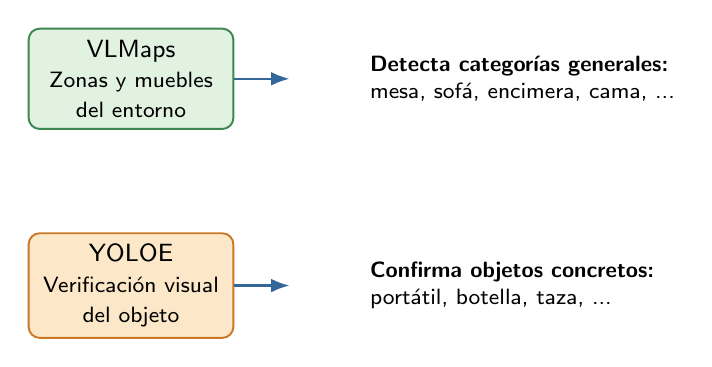
\begin{tikzpicture}[node distance=1.3cm and 1.6cm]
  \node[bloque, fill=figVerde, draw=figVerdeBorde] (vlmaps) {VLMaps\\\footnotesize Zonas y muebles\\\footnotesize del entorno};
  \node[right=of vlmaps, draw=none, fill=none, align=left, font=\sffamily\footnotesize] (vd) {%
    \textbf{Detecta categorías generales:}\\ mesa, sofá, encimera, cama, ...};
  \node[bloquen, below=of vlmaps] (yoloe) {YOLOE\\\footnotesize Verificación visual\\\footnotesize del objeto};
  \node[right=of yoloe, draw=none, fill=none, align=left, font=\sffamily\footnotesize] (yd) {%
    \textbf{Confirma objetos concretos:}\\ portátil, botella, taza, ...};
  \draw[flecha] (vlmaps.east) -- ($(vlmaps.east) + (0.7,0)$);
  \draw[flecha] (yoloe.east) -- ($(yoloe.east) + (0.7,0)$);
\end{tikzpicture}
\caption[Roles complementarios de VLMaps y YOLOE.]{Roles complementarios: el mapa semántico propone zonas plausibles y YOLOE confirma visualmente el objeto.}
\label{fig:vlmaps_yoloe}
\end{figure}

\paragraph{Flujo actual para objetos pequeños.} En las consultas del tipo ``ve a una habitación y encuentra un objeto'', el sistema no pregunta a VLMaps directamente por el objeto pequeño cuando este no suele estar representado de forma estable en el mapa. La instrucción se interpreta primero para separar habitación y objeto; si la habitación aparece explícitamente, queda fijada como restricción de búsqueda. Después, el objeto se normaliza en dos niveles: una etiqueta visual para YOLOE, usada en la confirmación, y una o varias categorías de soporte para VLMaps, usadas para generar puntos de exploración alrededor de muebles plausibles. Por ejemplo, una consulta sobre una botella se transforma en una búsqueda visual de \emph{bottle}, pero en VLMaps se apoya en zonas como \emph{counter}, \emph{table}, \emph{shelf} o \emph{cabinet}. En el caso de un libro, el soporte natural pasa por \emph{shelf}, \emph{desk} o \emph{table}.

Con esta separación, VLMaps actúa como generador de hipótesis espaciales y no como detector final. Sus mapas de calor se recortan a la habitación fijada, se fusionan entre las categorías de soporte y se convierten en puntos de exploración navegables alrededor de los muebles activados. Si no hay evidencia semántica útil dentro de la habitación, el sistema cae a una cobertura geométrica de la región navegable. Mientras el robot se desplaza, YOLOE se ejecuta de forma persistente sobre la cámara: un umbral bajo permite interrumpir la ruta cuando aparece una posible detección, y umbrales más altos se reservan para confirmar el objeto desde cerca. Este flujo se resume en la figura~\ref{fig:flujo_objetos_pequenos}.

\begin{figure}[H]
\centering
\resizebox{\linewidth}{!}{%
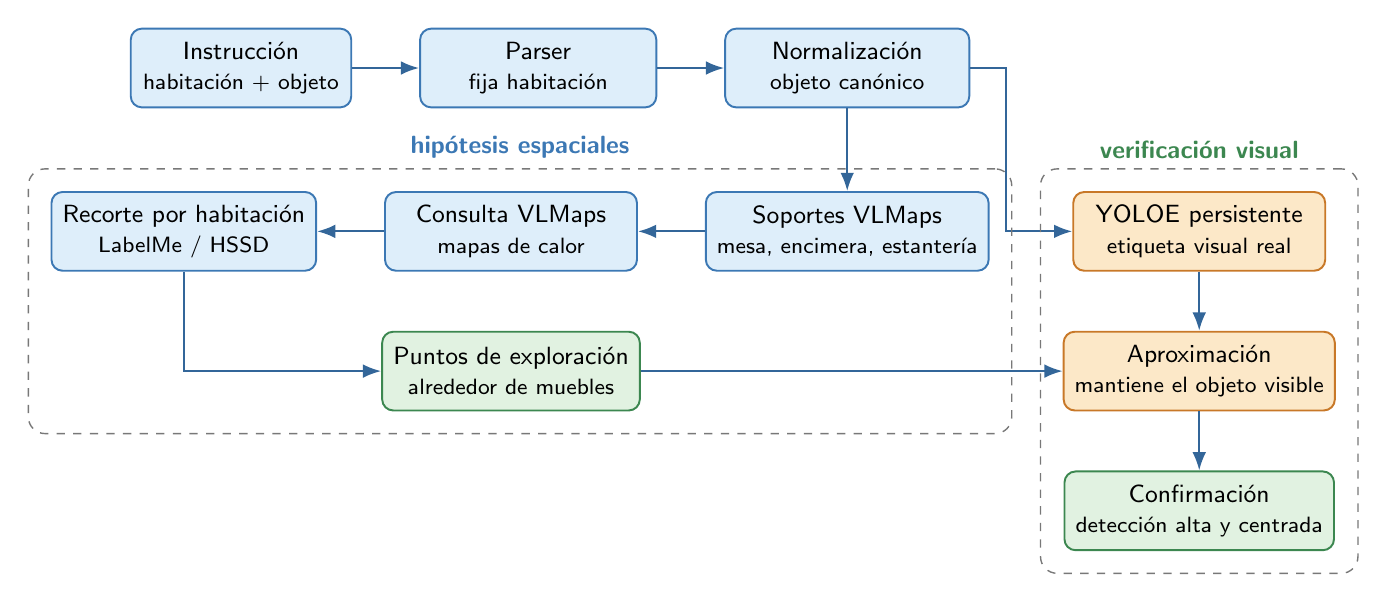
\begin{tikzpicture}[node distance=0.75cm and 0.85cm]
  \node[bloque, minimum width=2.8cm, minimum height=1.0cm] (query) {Instrucción\\\footnotesize habitación + objeto};
  \node[bloque, minimum width=3.0cm, minimum height=1.0cm, right=of query] (parse) {Parser\\\footnotesize fija habitación};
  \node[bloque, minimum width=3.1cm, minimum height=1.0cm, right=of parse] (resolve) {Normalización\\\footnotesize objeto canónico};

  \node[bloque, minimum width=3.2cm, minimum height=1.0cm, below=1.05cm of resolve] (support) {Soportes VLMaps\\\footnotesize mesa, encimera, estantería};
  \node[bloque, minimum width=3.2cm, minimum height=1.0cm, left=of support] (vlmaps) {Consulta VLMaps\\\footnotesize mapas de calor};
  \node[bloque, minimum width=3.2cm, minimum height=1.0cm, left=of vlmaps] (roommask) {Recorte por habitación\\\footnotesize LabelMe / HSSD};
  \node[bloquev, minimum width=3.2cm, minimum height=1.0cm, below=of vlmaps] (points) {Puntos de exploración\\\footnotesize alrededor de muebles};

  \node[bloquen, minimum width=3.2cm, minimum height=1.0cm, right=1.05cm of support] (yoloe) {YOLOE persistente\\\footnotesize etiqueta visual real};
  \node[bloquen, minimum width=3.2cm, minimum height=1.0cm, below=of yoloe] (approach) {Aproximación\\\footnotesize mantiene el objeto visible};
  \node[bloquev, minimum width=3.2cm, minimum height=1.0cm, below=of approach] (confirm) {Confirmación\\\footnotesize detección alta y centrada};

  \draw[flecha] (query) -- (parse);
  \draw[flecha] (parse) -- (resolve);
  \draw[flecha] (resolve) -- (support);
  \draw[flecha] (support) -- (vlmaps);
  \draw[flecha] (vlmaps) -- (roommask);
  \draw[flecha] (roommask) |- (points);
  \draw[flecha] (points) -- (approach);
  \draw[flecha] (resolve.east) -- ++(0.45,0) |- (yoloe.west);
  \draw[flecha] (yoloe) -- (approach);
  \draw[flecha] (approach) -- (confirm);

  \node[grupo, fit=(support) (vlmaps) (roommask) (points),
        label={[anchor=south, font=\sffamily\bfseries\small, text=figAzulBorde]north:hipótesis espaciales}] {};
  \node[grupo, fit=(yoloe) (approach) (confirm),
        label={[anchor=south, font=\sffamily\bfseries\small, text=figVerdeBorde]north:verificación visual}] {};
\end{tikzpicture}%
}
\caption[Flujo de consulta para objetos pequeños.]{Flujo de consulta para objetos pequeños: la orden se separa en habitación, soportes semánticos para VLMaps y etiqueta visual para YOLOE. VLMaps distribuye los puntos alrededor de muebles plausibles y YOLOE confirma el objeto real desde la cámara.}
\label{fig:flujo_objetos_pequenos}
\end{figure}

\paragraph{Mejora robusta simplificada.} A partir de las pruebas con objetos pequeños se añadió una mejora específica para evitar un fallo observado con libros y botellas: YOLOE puede detectar el objeto de forma intermitente y perderlo durante uno o varios frames justo cuando el robot empieza a acercarse. La versión final mantiene una arquitectura deliberadamente simple. VLMaps sigue proponiendo puntos de exploración alrededor de soportes plausibles dentro de la habitación; YOLOE confirma el objeto real desde la cámara; y, durante la aproximación, se acumula evidencia temporal en lugar de decidir por un único frame. Se probó una memoria visual proyectada con varias vistas alternativas, pero se descartó como comportamiento por defecto porque complicaba demasiado el circuito de exploración. En su lugar se conserva un único fallback planificado hacia el punto navegable más cercano a la última detección.

\begin{figure}[H]
\centering
\resizebox{\linewidth}{!}{%
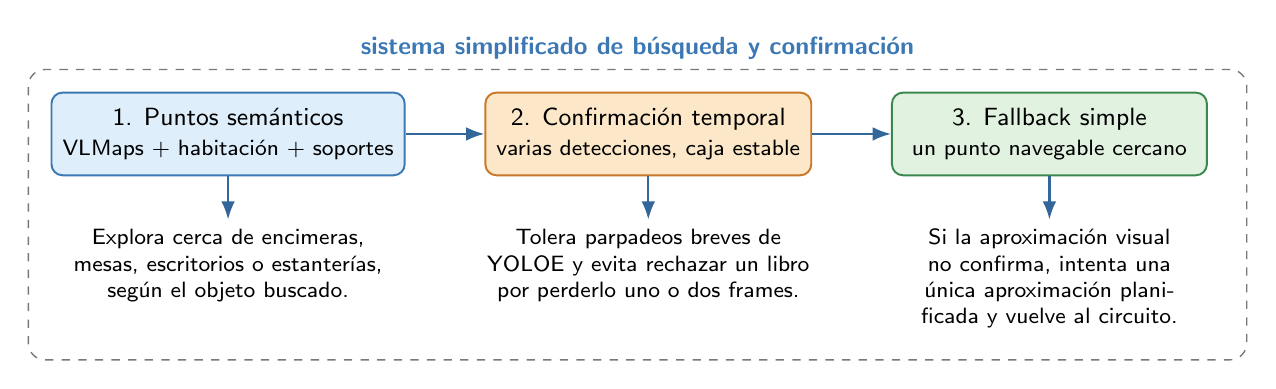
\begin{tikzpicture}[node distance=0.85cm and 1.0cm]
  \node[bloque, minimum width=4.0cm, minimum height=1.05cm] (sem) {1. Puntos semánticos\\\footnotesize VLMaps + habitación + soportes};
  \node[bloquen, minimum width=4.0cm, minimum height=1.05cm, right=of sem] (temp) {2. Confirmación temporal\\\footnotesize varias detecciones, caja estable};
  \node[bloquev, minimum width=4.0cm, minimum height=1.05cm, right=of temp] (fallback) {3. Fallback simple\\\footnotesize un punto navegable cercano};

  \node[draw=none, fill=none, below=0.55cm of sem, align=center, font=\sffamily\footnotesize, text width=4.2cm] (semTxt) {Explora cerca de encimeras, mesas, escritorios o estanterías, según el objeto buscado.};
  \node[draw=none, fill=none, below=0.55cm of temp, align=center, font=\sffamily\footnotesize, text width=4.2cm] (tempTxt) {Tolera parpadeos breves de YOLOE y evita rechazar un libro por perderlo uno o dos frames.};
  \node[draw=none, fill=none, below=0.55cm of fallback, align=center, font=\sffamily\footnotesize, text width=4.2cm] (fallbackTxt) {Si la aproximación visual no confirma, intenta una única aproximación planificada y vuelve al circuito.};

  \draw[flecha] (sem) -- (temp);
  \draw[flecha] (temp) -- (fallback);
  \draw[flecha] (sem) -- (semTxt);
  \draw[flecha] (temp) -- (tempTxt);
  \draw[flecha] (fallback) -- (fallbackTxt);

  \node[grupo, fit=(sem) (temp) (fallback) (semTxt) (tempTxt) (fallbackTxt),
        label={[anchor=south, font=\sffamily\bfseries\small, text=figAzulBorde]north:sistema simplificado de búsqueda y confirmación}] {};
\end{tikzpicture}%
}
\caption[Mejora robusta simplificada.]{Mejora robusta simplificada para objetos pequeños: VLMaps propone puntos cerca de soportes plausibles, YOLOE confirma con evidencia temporal y el planificador mantiene un único fallback navegable antes de continuar la exploración.}
\label{fig:mejora_simplificada}
\end{figure}

\subsection*{Verificación visual con YOLOE}

Para cubrir esa limitación se integró el detector visual \textbf{YOLOE}~\cite{wang2025yoloe}, capaz de comprobar en la imagen de la cámara si aparece un objeto descrito por una etiqueta textual. Su papel no es sustituir al mapa semántico, sino cerrar la cadena de decisión: la capa semántica propone una zona plausible y YOLOE confirma, desde una vista concreta, si el objeto está realmente presente.

Durante la integración apareció un problema técnico importante. La ejecución del detector dentro del mismo proceso que el simulador provocaba conflictos entre la GPU y la tecnología gráfica utilizada por Habitat-Sim para mostrar la escena. Para resolverlo, la detección se desplazó a un proceso separado: el proceso principal guarda la imagen, lanza el detector aparte y recupera el resultado en un formato estructurado. Esta solución hizo posible mantener la simulación estable durante la verificación visual y separar de forma clara las responsabilidades de cada componente.

Sobre la verificación se añadió un \textbf{escaneo multiángulo}. En lugar de evaluar una sola imagen frontal, el robot realiza pequeñas rotaciones laterales y repite la detección. Esta decisión responde a una limitación práctica: en interiores, un objeto puede estar presente pero quedar parcialmente oculto o fuera del encuadre desde una única pose.

\subsection*{Mejora de candidatos y navegación}

Con el detector operativo, el siguiente problema fue la calidad de los candidatos extraídos del mapa semántico. El mapa de calor que produce esa capa puede contener ruido, regiones pequeñas o activaciones situadas al otro lado de una pared. Si se navega directamente hacia esas regiones, el sistema falla aunque el detector visual funcione correctamente.

Para reducir ese problema se aplicaron filtros consecutivos: coherencia global del mapa de calor, tamaño mínimo de región y descarte de candidatos separados por pared. En paralelo, se reforzó la planificación de trayectoria, la detección de colisiones, la replanificación y el uso de varios candidatos. Estas mejoras no cambian la fuente semántica, pero evitan que una buena decisión de alto nivel se pierda por una navegación hacia una región geométricamente inviable.

\paragraph{Procesado del mapa de calor en detalle.} El procesado real, tal como está implementado, se organiza en dos fases bien diferenciadas que se resumen en la figura~\ref{fig:heatmap_pipeline}. La primera fase \emph{construye} el mapa de calor crudo a partir de las puntuaciones del mapa semántico, y la segunda lo \emph{limpia} para que solo lleguen a la navegación zonas consistentes.

\begin{figure}[H]
\centering
\resizebox{0.96\linewidth}{!}{%
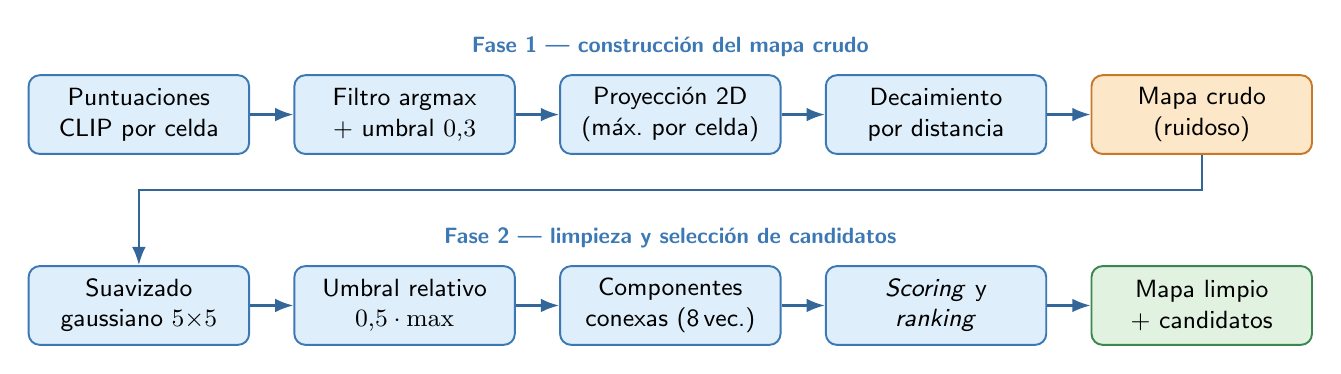
\begin{tikzpicture}[node distance=0.45cm and 0.55cm]
  % Fase 1: construcción del mapa crudo
  \node[bloque, minimum width=2.8cm, minimum height=1.0cm] (clip) {Puntuaciones\\CLIP por celda};
  \node[bloque, minimum width=2.8cm, minimum height=1.0cm, right=of clip] (argm) {Filtro argmax\\+ umbral $0{,}3$};
  \node[bloque, minimum width=2.8cm, minimum height=1.0cm, right=of argm] (proj) {Proyección 2D\\(máx.\ por celda)};
  \node[bloque, minimum width=2.8cm, minimum height=1.0cm, right=of proj] (dist) {Decaimiento\\por distancia};
  \node[bloquen, minimum width=2.8cm, minimum height=1.0cm, right=of dist] (raw) {Mapa crudo\\(ruidoso)};

  \draw[flecha] (clip) -- (argm);
  \draw[flecha] (argm) -- (proj);
  \draw[flecha] (proj) -- (dist);
  \draw[flecha] (dist) -- (raw);

  % Etiqueta de fase 1
  \node[font=\sffamily\bfseries\footnotesize, text=figAzulBorde, above=0.1cm of proj]
        {Fase 1 — construcción del mapa crudo};

  % Fase 2: limpieza
  \node[bloque, minimum width=2.8cm, minimum height=1.0cm, below=1.4cm of clip] (blur) {Suavizado\\gaussiano $5{\times}5$};
  \node[bloque, minimum width=2.8cm, minimum height=1.0cm, right=of blur] (thr) {Umbral relativo\\$0{,}5\cdot\max$};
  \node[bloque, minimum width=2.8cm, minimum height=1.0cm, right=of thr] (cc) {Componentes\\conexas (8\,vec.)};
  \node[bloque, minimum width=2.8cm, minimum height=1.0cm, right=of cc] (score) {\textit{Scoring} y\\\textit{ranking}};
  \node[bloquev, minimum width=2.8cm, minimum height=1.0cm, right=of score] (clean) {Mapa limpio\\+ candidatos};

  \draw[flecha] (blur) -- (thr);
  \draw[flecha] (thr) -- (cc);
  \draw[flecha] (cc) -- (score);
  \draw[flecha] (score) -- (clean);

  \node[font=\sffamily\bfseries\footnotesize, text=figAzulBorde, above=0.1cm of cc]
        {Fase 2 — limpieza y selección de candidatos};

  % Conexión entre fases
  \draw[flecha] (raw.south) -- ++(0,-0.45) -| (blur.north);
\end{tikzpicture}%
}
\caption[Procesado en dos fases del mapa de calor.]{Procesado en dos fases del mapa de calor: construcción del mapa crudo y limpieza para extraer candidatos.}
\label{fig:heatmap_pipeline}
\end{figure}

\subparagraph{Fase 1 — construcción del mapa crudo.} Se parte de la matriz de puntuaciones CLIP del mapa semántico. CLIP es un modelo de visión-lenguaje que, para cada celda~$x$ del entorno, asigna una puntuación~$s_c(x)$ por cada categoría visual~$c$ (mesa, cama, sofá, ventana, etc.); cuanto más alta la puntuación, más se parece esa zona del entorno a la categoría. Para la categoría buscada~$c^{*}$ (por ejemplo, \emph{cama}) se conserva la puntuación solo si esa categoría es la dominante en la celda y supera un umbral mínimo:
%
\begin{equation}
\tilde s(x) =
\begin{cases}
s_{c^{*}}(x) & \text{si } \arg\max_{c} s_c(x) = c^{*} \text{ y } s_{c^{*}}(x) > t_0,\\
0 & \text{en otro caso,}
\end{cases}
\qquad t_0 = 0{,}3.
\label{eq:argmax_filter}
\end{equation}
%
\emph{Lectura intuitiva:} el operador $\arg\max$ devuelve, de entre todas las categorías, la que tiene la puntuación más alta en esa celda. La condición $\arg\max_c s_c(x) = c^{*}$ se traduce como: ``en esta celda, \emph{cama} es la categoría que más se parece, no solo una de las que algo se parece''. Así evitamos quedarnos con zonas ambiguas que disparan a la vez \emph{cama} y \emph{sofá}. El umbral $t_0=0{,}3$ descarta además celdas donde incluso la mejor categoría tiene poca confianza. Después, las puntuaciones que sobreviven se proyectan a una rejilla 2D vista desde arriba, quedándose con el máximo por casilla: distintas alturas de una misma columna del espacio 3D se colapsan a un único valor.

Para evitar un mapa puramente formado por puntos aislados, las celdas \emph{vecinas} a las activaciones se rellenan con un \textbf{decaimiento por distancia}, en el que el valor disminuye linealmente y se trunca a cero por debajo de un mínimo:
%
\begin{equation}
h_{\text{crudo}}(x) =
\begin{cases}
\tilde s(x) & \text{si } \tilde s(x) > 0,\\
\max\bigl(1 - 0{,}3 \cdot d(x),\,0\bigr) \cdot \mathbf{1}[\cdot \geq 0{,}15] & \text{en otro caso,}
\end{cases}
\label{eq:dist_decay}
\end{equation}
%
donde $d(x)$ es la distancia (en celdas) a la celda activa más próxima. \emph{Lectura intuitiva:} alrededor de una activación válida pintamos un halo cuyo valor cae con la distancia hasta apagarse. Si $d=1$ el valor es $0{,}7$; si $d=3$ es $0{,}1$ y se trunca a cero por estar bajo $0{,}15$. Esto da continuidad espacial al mapa y permite que las regiones aparezcan como ``manchas'' en lugar de píxeles sueltos. De esta fase sale un mapa continuo pero ruidoso, con muchas activaciones espurias.

\subparagraph{Fase 2 — limpieza y selección de candidatos.} Sobre $h_{\text{crudo}}$ se aplica un \textbf{suavizado gaussiano}. Un filtro gaussiano 2D es un núcleo de convolución de la forma
%
\begin{equation}
G_\sigma(x,y) = \frac{1}{2\pi\sigma^{2}}\,
\exp\!\left(-\frac{x^{2}+y^{2}}{2\sigma^{2}}\right),
\label{eq:gauss}
\end{equation}
%
\emph{Lectura intuitiva:} esta fórmula describe la conocida ``campana de Gauss'' en dos dimensiones, centrada en el origen, con su pico en el centro y caída suave hacia los lados controlada por~$\sigma$. Al convolucionar el mapa con esta campana, cada celda pasa a ser una media ponderada de ella misma y de sus vecinas, dando más peso a las más próximas. Esta operación se conoce como \emph{filtro paso-bajo} porque deja pasar la información ``lenta'' (las regiones grandes y continuas) y atenúa la información ``rápida'' (el ruido aislado y los bordes muy abruptos). Es importante que el contorno general de las regiones no se desplace: solo se afinan los bordes y se eliminan chispazos sueltos. Aquí se usa un núcleo $5\times 5$ con $\sigma=1$ celda. Llamando $H = G_\sigma * h_{\text{crudo}}$ al mapa suavizado, se binariza con un \textbf{umbral relativo}:
%
\begin{equation}
M(x) = \mathbf{1}\bigl[\,H(x) \geq \alpha\cdot\max_{y} H(y)\,\bigr],
\qquad \alpha = 0{,}5.
\label{eq:rel_threshold}
\end{equation}
%
\emph{Lectura intuitiva:} la función indicadora $\mathbf{1}[\cdot]$ vale 1 si la condición se cumple y 0 si no, de modo que $M(x)$ es una máscara que dice ``aquí sí, aquí no''. La condición es ``el valor de esta celda llega al menos a la mitad del valor más alto de toda la escena''. Se usa umbral \emph{relativo} y no absoluto porque escenas con activaciones débiles seguirían vacías con un umbral fijo: $\alpha = 0{,}5$ exige que cada celda valga al menos la mitad del máximo de la escena, sea cual sea ese máximo.

Sobre la máscara $M$ se calculan las \textbf{componentes conexas} con conectividad de 8 vecinos: dos celdas activas pertenecen a la misma región si comparten un lado o una esquina. Es la forma estándar de agrupar píxeles que ``están juntos'' en una imagen binaria. Cada componente $i$ tiene un área $a_i$ (en celdas), una intensidad media $\bar v_i$, una intensidad máxima $v^{\max}_i$ y una suma $S_i$ (suma de todos los valores dentro de la región). Se descartan las componentes con $a_i < 3$ porque suelen ser ruido, y al resto se les asigna una puntuación mediante
%
\begin{equation}
s_i = \bar v_i \cdot \log(1 + a_i).
\label{eq:component_score}
\end{equation}
%
\emph{Lectura intuitiva:} multiplicamos cuánto se parece la región a la categoría (intensidad media) por una versión ``apaciguada'' de su tamaño. El logaritmo es el truco: el área pesa, pero su efecto crece muy despacio ---una región de 100 celdas no puntúa 100 veces más que una de una sola celda, sino unas 5 veces más---. Así una mancha enorme no aplasta a otra mediana solo por ser grande, pero una mancha minúscula tampoco gana solo por ser muy intensa. Una región se conserva si su puntuación es competitiva con la mejor:
%
\begin{equation}
s_i \;\geq\; \rho \cdot \max_{j} s_j,\qquad \rho = 0{,}2,
\label{eq:keep_ratio}
\end{equation}
%
es decir, sobreviven las componentes que llegan al menos al 20\,\% de la puntuación de la mejor; el resto se considera ruido. Por último, las supervivientes se reordenan por una métrica de calidad final que combina área, intensidad media y suma, con cada término normalizado a su máximo entre las componentes conservadas:
%
\begin{equation}
q_i = 0{,}20\,\frac{a_i}{a^{\max}} \;+\; 0{,}35\,\bar v_i \;+\; 0{,}45\,\frac{S_i}{S^{\max}}.
\label{eq:quality}
\end{equation}
%
\emph{Lectura intuitiva:} es una nota final ponderada en la que la suma normalizada pesa más (45\,\%) porque captura a la vez ``tamaño y energía'': una región grande y razonablemente intensa acumula mucha suma; una región pequeña pero muy brillante no llega. La intensidad media (35\,\%) refleja cuán fuerte es la señal, y el área (20\,\%) garantiza que las regiones de tamaño real no pierdan frente a chispazos. Esta puntuación final evita el caso típico de ruido en el que un blob diminuto y muy intenso gana a una región del tamaño de un sofá con intensidad razonable.

La salida son: un mapa limpio con ceros fuera de las componentes retenidas, una máscara booleana y la lista ordenada de componentes con su \emph{bounding box} (rectángulo que las contiene) y centroide. El descarte de candidatos separados por pared no forma parte de esta función: lo aplica después la capa de navegación, comprobando si el centroide cae sobre una celda navegable del mapa de ocupación.

\paragraph{Cálculo de trayectorias y evitación de colisiones.} Una vez seleccionado el candidato, hace falta una trayectoria que lleve al robot hasta él sin chocar con las paredes ni con el mobiliario. Aquí intervienen dos piezas que comparten el mismo mapa de ocupación pero juegan papeles distintos: el \emph{planificador global}, que dibuja el camino antes de moverse, y el \emph{escudo local}, que vigila durante la ejecución.

El planificador trabaja sobre una versión del mapa con los obstáculos \emph{dilatados}: se hinchan tres iteraciones (unos 15\,cm por lado) para incluir un margen de seguridad equivalente al ancho del robot. Sobre ese mapa dilatado se construye un grafo de visibilidad (\emph{visibility graph}, PyVisGraph) cuyos nodos son las esquinas convexas del espacio libre y cuyas aristas son los segmentos rectos que no atraviesan obstáculos. Las rutas se trazan con un algoritmo $A^{\!*}$ \emph{clearance-aware}, una variante del clásico $A^{\!*}$ que, además del coste por longitud, penaliza pasar cerca de obstáculos. La función \texttt{plan\_path\_only()} permite calcular y previsualizar el camino sin ejecutarlo, lo que resultó útil para detectar rutas dudosas antes de mover el robot.

La calidad de cada ruta se mide a posteriori con una métrica de seguridad basada en la \emph{transformada de distancias} (\texttt{distance\_transform\_edt}), que para cada celda calcula la distancia al obstáculo más cercano. Para un camino dado se registran la holgura mínima, la holgura media, la longitud y un coste compuesto $\text{longitud} + 0{,}5\cdot\text{penalización}$, donde la penalización suma una unidad por cada celda con menos de 8 de holgura. Si la holgura mínima del trayecto cae por debajo de un umbral (\texttt{MIN\_PATH\_CLEARANCE}~$=1$ celda) o el destino mismo tiene poca holgura (\texttt{MIN\_GOAL\_CLEARANCE}~$=3$ celdas), el sistema descarta la ruta y prueba con candidatos alternativos; si ninguno cumple, la consulta se omite. La seguridad es así una puerta de control, no una nota informativa.

Para que el destino caiga siempre en un sitio razonable, el centroide de la componente del mapa de calor se proyecta a un \emph{anillo de aproximación}: se muestrean posiciones a entre 8 y 25 celdas alrededor del centroide, se filtran las navegables y, dentro de ellas, se elige la de mayor holgura y proximidad al robot (\texttt{find\_safe\_candidate\_approach\_goals}). Si el destino es una habitación en lugar de un objeto, se aplica el equivalente \texttt{find\_reachable\_room\_goal}, que enumera todas las celdas navegables del polígono de la habitación y devuelve las más seguras. En ambos casos, si el punto elegido no es navegable, se ``imanta'' a la celda libre más próxima con \texttt{\_snap\_to\_nearest\_free()}, una operación basada otra vez en la transformada de distancias. Estos detalles evitan dos fallos clásicos: planificar contra un centroide que cae dentro de un obstáculo, y declarar que se ha llegado a una habitación cuando en realidad se ha terminado en otra adyacente.

Durante la ejecución, un \textbf{escudo local de colisiones} vigila cada acción \texttt{move\_forward}. Antes de avanzar, predice la celda siguiente a partir de la posición y orientación actuales del robot y consulta su holgura en el mapa de ocupación crudo (sin dilatar). Si esa holgura es menor que \texttt{STOP\_CL}~$=1$ celda, la ejecución se interrumpe; si está entre \texttt{STOP\_CL} y \texttt{SLOW\_CL}~$=2{,}5$ celdas, se emite un aviso pero no se detiene el movimiento. La asimetría entre planificador y escudo --- mapa dilatado para planificar, mapa crudo para vigilar --- es deliberada: la dilatación asegura rutas con margen, mientras que el escudo trabaja sobre el espacio físico real y permite cruzar pasillos estrechos sin disparar paradas falsas. El resultado es una navegación \emph{one-shot}: se planifica una vez, se ejecuta una vez y se reporta el estado final del robot, sin reintentos opacos que dificultarían después la evaluación.

\subsection*{Razonamiento por habitaciones}

Este bloque constituye la aportación principal del proyecto. Una vez consolidado el flujo funcional, se observó una limitación de fondo: buscar directamente sobre el mapa semántico ordena candidatos por afinidad global, pero no razona como lo haría una persona. Para encontrar una botella, por ejemplo, no se inspecciona cualquier punto activado del mapa; primero se piensa en cocina, comedor o zonas de almacenamiento, y después en mesas, encimeras o estanterías.

La hipótesis de esta fase es que una búsqueda jerárquica, organizada como habitación, zona o mueble y objeto concreto, es más interpretable y potencialmente más eficiente que una búsqueda plana sobre el mapa. La figura~\ref{fig:razonamiento_habitaciones} muestra los tres niveles que rigen el comportamiento del sistema.

\begin{figure}[h]
\centering
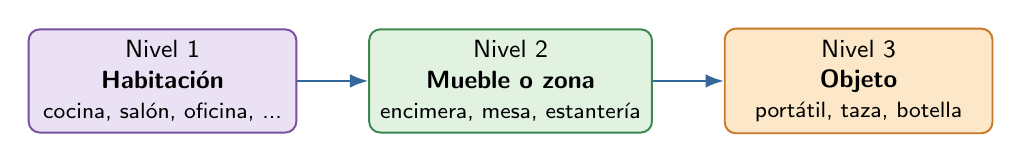
\begin{tikzpicture}[node distance=0.6cm and 0.9cm]
  \node[bloquei, minimum width=3.4cm] (h) {Nivel 1\\\textbf{Habitación}\\\footnotesize cocina, salón, oficina, ...};
  \node[bloquev, right=of h, minimum width=3.4cm] (m) {Nivel 2\\\textbf{Mueble o zona}\\\footnotesize encimera, mesa, estantería};
  \node[bloquen, right=of m, minimum width=3.4cm] (o) {Nivel 3\\\textbf{Objeto}\\\footnotesize portátil, taza, botella};
  \draw[flecha] (h) -- (m);
  \draw[flecha] (m) -- (o);
\end{tikzpicture}
\caption[Tres niveles del razonamiento de búsqueda.]{Tres niveles del razonamiento: habitación, zona o mueble y objeto.}
\label{fig:razonamiento_habitaciones}
\end{figure}

Para implementar esta idea, se sustituyó el entorno principal de pruebas. \textbf{HSSD}~\cite{khanna2024hssd} pasó a ser el conjunto de escenas de referencia y Matterport3D quedó como soporte secundario. La razón es que HSSD incluye anotaciones nativas de habitaciones, lo que resulta esencial para poder evaluar el razonamiento jerárquico. Este enfoque jerárquico se alinea con propuestas recientes de búsqueda interactiva guiada por lenguaje~\cite{honerkamp2024moma}.

Sobre esa base se desarrollaron tres componentes muy ligados entre sí. En primer lugar, un \textbf{proveedor de habitaciones}, que aprovecha las anotaciones de HSSD para asociar cada celda del mapa a una habitación concreta y recuperar información básica de su estructura. En segundo lugar, un \textbf{estado estructurado de búsqueda}, que registra, para cada habitación, el grado de exploración, los candidatos probados, los objetos observados y la relevancia respecto al objetivo actual. Por último, un \textbf{selector de habitación}, integrado en el flujo de ejecución, que decide qué habitación conviene inspeccionar antes de elegir un candidato concreto.

Con estos componentes, el sistema deja de ser un buscador plano sobre el mapa y pasa a ser un buscador jerárquico basado en habitaciones. Esta arquitectura facilita además una evaluación más interpretable: permite medir si la primera habitación elegida era razonable, cuántas habitaciones se visitaron antes del éxito y cuántos candidatos se inspeccionaron sin confirmar el objeto.

\subsection*{Evaluación inicial y análisis de comportamiento}

Una vez consolidada la arquitectura, se planteó una primera fase de análisis comparativo. El objetivo era comprobar dos decisiones: si conviene utilizar el mapa de calor semántico directamente o filtrarlo antes de seleccionar candidatos, y si la búsqueda debe permanecer integrada en el flujo de navegación o organizarse como un ejecutor de acciones de alto nivel.

Estos análisis se realizaron durante las prácticas en un volumen reducido y de forma cualitativa, con consultas representativas dentro del contenedor de simulación. El resultado no fue una conclusión cerrada, sino una lectura útil del estado del sistema: el método base se mostró más estable en las pruebas realizadas, mientras que el ejecutor aportó una estructura más clara y mejor preparada para depuración y evaluación futura.

%----------------------------------------------------------------------------------------
%	CAPÍTULO 3: RESUMEN DE RESULTADOS
%----------------------------------------------------------------------------------------

\chapter{Resumen de Resultados}\label{chap:resultados}

Tras varias semanas de integración y refinamiento, el sistema pasó de una base de simulación a una arquitectura funcional de búsqueda semántica. El resultado principal no es un detector aislado ni una ruta concreta, sino una cadena completa de decisión: interpretar la orden, elegir una habitación plausible, seleccionar una zona semántica, navegar hasta ella y confirmar visualmente el objeto. Los resultados descritos en este capítulo corresponden a las 150 horas de la asignatura IR2137 y a las tareas representadas en el diagrama de Gantt.

\section{Resultados obtenidos}

A lo largo del proyecto se completaron varios objetivos técnicos. Se presentan ordenados por bloque para mantener la progresión real del trabajo.

\paragraph{Entorno reproducible de desarrollo.} Se configuró un entorno aislado mediante Docker y CUDA, capaz de reproducir las condiciones de ejecución del proyecto en distintas máquinas. Esta base redujo los problemas de dependencias y permitió separar navegación, simulación, mapas semánticos y ejecución de pruebas.

\paragraph{Simulación funcional con Habitat-Sim.} Se dejó operativa una primera versión de navegación en escenas de Matterport3D. Aunque todavía no incorporaba el razonamiento jerárquico, sirvió como banco de pruebas para validar sensores, movimiento y planificación.

\paragraph{Integración de VLMaps como mapa semántico.} La herramienta se incorporó para asociar regiones del mapa con categorías de mobiliario y zonas relevantes. Su utilidad quedó clara para proponer dónde buscar, pero también se comprobó su limitación: no confirma objetos pequeños. Esta observación justificó separar propuesta semántica y confirmación visual.

\paragraph{Verificación visual con YOLOE.} Se integró YOLOE como verificador final. La detección se separó en un proceso independiente para evitar conflictos entre el simulador y la GPU, y se añadió un escaneo multiángulo para reducir falsos negativos cuando el objeto no aparece bien encuadrado desde una sola vista.

\paragraph{Mejora de la calidad de candidatos.} Sobre el mapa de calor original se aplicaron filtros de coherencia global, tamaño de región y pared. Junto con la planificación, la detección de colisiones y la replanificación, estos filtros redujeron candidatos geométricamente inviables. También se incorporó el modelo de lenguaje para sugerir categorías y habitaciones probables a partir del objeto buscado.

\paragraph{Razonamiento por habitaciones.} El proyecto se reorganizó como una búsqueda jerárquica de tres niveles: habitación, mueble o zona y objeto concreto. HSSD pasó a ser el entorno principal por sus anotaciones nativas de habitaciones, y se implementaron el proveedor de habitaciones, el estado estructurado de búsqueda y el selector de habitación. Esta capa constituye la aportación principal del periodo.

\paragraph{Comparaciones iniciales.} Dentro de las horas de prácticas se realizaron primeras comparaciones entre dos pares de variantes: mapa de calor original frente a mapa de calor mejorado y método base frente a ejecutor estructurado. Sobre un conjunto reducido de consultas representativas se midieron unas pocas métricas, deliberadamente simples para que el resultado fuera interpretable, antes de extraer una lectura cualitativa que justificara el diseño final.

\medskip

\textbf{Métricas utilizadas.} Para los mapas de calor se consideran tres indicadores comprensibles: el \emph{porcentaje de candidato válido}, es decir, qué fracción de los candidatos seleccionados conduce a un punto realmente navegable; el \emph{tamaño medio del candidato} en celdas del mapa, que mide si las regiones propuestas son consistentes en lugar de pequeños fragmentos ruidosos; y el \emph{número medio de candidatos por consulta}, que indica cuánto se reduce la lista a inspeccionar tras el filtrado. Para la comparación entre método base y ejecutor se utilizan tres métricas habituales en búsqueda de objetos: la \emph{tasa de acierto global}, que es el porcentaje de consultas en las que el objeto se confirma con YOLOE; el \emph{acierto en la primera habitación}, que mide cuántas veces la habitación elegida en primer lugar contiene realmente el objeto; y el \emph{número medio de habitaciones visitadas} antes de cerrar la búsqueda.

\begin{table}[H]
\centering
\renewcommand{\arraystretch}{1.3}
\setlength{\tabcolsep}{6pt}
\begin{tabular}{>{\raggedright\arraybackslash}p{6.4cm}cc}
\toprule
\rowcolor{ocre!12}
\textbf{Métrica} & \textbf{Mapa original} & \textbf{Mapa mejorado}\\
\midrule
Porcentaje de candidato válido (\%)        & 71 & 88 \\
\midrule
Tamaño medio del candidato (celdas)        & 18 & 34 \\
\midrule
Candidatos por consulta (media)            & 6{,}4 & 3{,}1 \\
\bottomrule
\end{tabular}
\caption[Resultados cuantitativos sobre los mapas de calor.]{Resultados cuantitativos sobre los mapas de calor.}
\label{tab:cuant_mapa}
\end{table}

\begin{table}[H]
\centering
\renewcommand{\arraystretch}{1.3}
\setlength{\tabcolsep}{6pt}
\begin{tabular}{>{\raggedright\arraybackslash}p{6.4cm}cc}
\toprule
\rowcolor{ocre!12}
\textbf{Métrica} & \textbf{Método base} & \textbf{Ejecutor}\\
\midrule
Tasa de acierto global (\%)                & 56 & 49 \\
\midrule
Acierto en la primera habitación (\%)      & 61 & 67 \\
\midrule
Habitaciones visitadas antes del éxito     & 1{,}6 & 2{,}1 \\
\bottomrule
\end{tabular}
\caption[Resultados cuantitativos del ejecutor frente al método base.]{Resultados cuantitativos del ejecutor frente al método base.}
\label{tab:cuant_ejec}
\end{table}

Estos números se obtienen sobre un conjunto reducido de consultas dentro del periodo de prácticas, por lo que se interpretan como una primera lectura más que como resultados definitivos. Aun así, dan una base para la lectura cualitativa que recoge la tabla~\ref{tab:comparacion_metodos}, en la que se traduce el comportamiento observado a aspectos prácticos como estabilidad, organización de la búsqueda y candidatos incorrectos.

\begin{table}[H]
\centering
\renewcommand{\arraystretch}{1.35}
\setlength{\tabcolsep}{8pt}
\begin{tabular}{>{\raggedright\arraybackslash}p{3.0cm}
                 >{\raggedright\arraybackslash}p{4.6cm}
                 >{\raggedright\arraybackslash}p{4.8cm}}
\toprule
\rowcolor{ocre!12}
\textbf{Aspecto} & \textbf{Mapa mejorado vs. original} & \textbf{Ejecutor vs. método base}\\
\midrule
Estabilidad &
Comportamiento más limpio en escenas con ruido del mapa. &
El método base se mostró más estable en las pruebas realizadas. \\
\midrule
Organización &
Mejor selección inicial de la zona candidata en algunas escenas. &
El ejecutor organiza la búsqueda como acciones de alto nivel más legibles. \\
\midrule
Candidatos incorrectos &
Se reducen las regiones poco fiables. &
El ejecutor todavía inspecciona más candidatos incorrectos. \\
\midrule
Observación &
La mejora no es uniforme; depende de la escena. &
Arquitectura prometedora, requiere ajuste fino. \\
\bottomrule
\end{tabular}
\caption[Comparación cualitativa entre las versiones del sistema.]{Comparación cualitativa entre las versiones del sistema.}
\label{tab:comparacion_metodos}
\end{table}

Tomando ambas tablas en conjunto, el postprocesado del mapa de calor mejora la calidad de los candidatos de forma clara, aunque la mejora no es uniforme entre escenas. La comparación entre método base y ejecutor muestra una conclusión importante: estructurar mejor la búsqueda no garantiza por sí solo más aciertos (el método base aún supera al ejecutor en tasa global), pero sí mejora el acierto en la primera habitación y hace el comportamiento más interpretable y depurable. Esta lectura se utiliza como punto de partida para la evaluación cuantitativa más amplia prevista en el TFG.

\paragraph{Arquitectura preparada para la continuidad.} Como cierre del periodo, la capa semántica quedó aislada del resto del sistema y lista para conectarse a un entorno robótico más completo. El detalle de esa migración y de la organización en dos contenedores se aborda en el capítulo~\ref{chap:tfg}.

\section{Equipos y recursos utilizados}

El proyecto se ha apoyado en un conjunto reducido y coherente de herramientas, seleccionadas por su compatibilidad con el flujo de trabajo del laboratorio y por su uso habitual en investigación. A continuación se describen los principales recursos, agrupados por función.

\paragraph{Recursos de desarrollo.}

\textbf{Ordenador con sistema operativo Linux.} El equipo de trabajo es el habitual en investigación en robótica y visión por computador, con sistema operativo Linux. Sobre él se ejecutan tanto el simulador como los modelos visuales y de lenguaje.

\textbf{GPU y CUDA.} Permiten acelerar los modelos visuales utilizados en la simulación, el mapa semántico y la verificación visual. La aceleración por GPU es necesaria para que estos componentes se ejecuten a un ritmo razonable durante las pruebas.

\textbf{Docker.} Se utiliza como tecnología de contenedores para asegurar que el sistema se ejecuta en condiciones similares en distintas máquinas. Ayuda a separar el entorno semántico del entorno de navegación robótica, evitando conflictos entre dependencias.

\textbf{Python y Git.} Python es el lenguaje principal del proyecto, en el que están escritas las distintas piezas del sistema. Git se utiliza como sistema de control de versiones para registrar el avance del trabajo y mantener una historia ordenada de los cambios.

\paragraph{Recursos de datos y simulación.}

\textbf{Habitat-Sim.} Simulador 3D utilizado durante todo el proyecto para mover un robot virtual por escenas interiores y probar el flujo de navegación. Permite trabajar de forma reproducible con sensores virtuales antes de pasar a un robot físico o a otro simulador.

\textbf{Matterport3D.} Conjunto de escenas interiores reconstruidas a partir de datos reales. Se utiliza como entorno de pruebas inicial y, una vez consolidada la capa de habitaciones, queda como soporte secundario.

\textbf{HSSD.} Conjunto de escenas sintéticas con anotaciones nativas de habitaciones. Es la base del razonamiento por habitaciones del proyecto y, durante las prácticas, se convierte en el entorno principal de pruebas.

\paragraph{Recursos semánticos y visuales.}

\textbf{VLMaps.} Herramienta de mapa semántico que relaciona zonas del entorno con categorías generales. Se apoya en modelos de visión-lenguaje y, en este proyecto, actúa como memoria semántica del entorno.

\textbf{YOLOE.} Detector visual de vocabulario abierto. Se utiliza como verificador final de la búsqueda, comprobando con la cámara del robot si el objeto solicitado está realmente presente.

\textbf{Modelo de lenguaje.} Se emplea para interpretar la instrucción, traducir el objeto buscado a categorías del mapa semántico y sugerir habitaciones probables. Su uso se limita a tareas de comprensión y enriquecimiento semántico, no a tomar decisiones de bajo nivel.

\paragraph{Recursos preparados para la continuidad.}

\textbf{ROS 1 Noetic.} Conjunto de herramientas estándar en robótica, utilizado durante el periodo de prácticas únicamente para preparar la migración inicial. La integración completa se desarrolla en el TFG.

\textbf{Gazebo y RViz.} Simulador robótico y herramienta de visualización asociados a ROS. Quedan integrados con el contenedor de simulación robótica para futuras pruebas de navegación.

\textbf{rosbridge.} Puente de comunicación que permite que el contenedor semántico hable con el contenedor de ROS sin compartir el mismo proceso.

\paragraph{Apoyo puntual con herramientas asistidas.} En tareas mecánicas y repetitivas, como adaptar ficheros de configuración o preparar archivos de arranque dentro de la migración a ROS, se utilizó de forma puntual Claude Code como asistente. Las decisiones técnicas, la validación de resultados y la revisión del comportamiento del sistema fueron, en cualquier caso, responsabilidad propia.

La figura~\ref{fig:herramientas} agrupa todos estos recursos por función, para dar una visión global de cómo se combinan.

\begin{figure}[h]
\centering
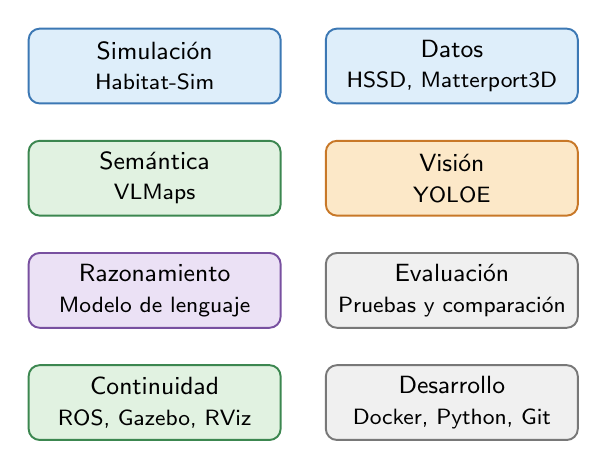
\begin{tikzpicture}[node distance=0.45cm and 0.55cm]
  \node[bloque, minimum width=3.2cm] (sim) {Simulación\\\footnotesize Habitat-Sim};
  \node[bloque, right=of sim, minimum width=3.2cm] (data) {Datos\\\footnotesize HSSD, Matterport3D};
  \node[bloquev, below=of sim, minimum width=3.2cm] (sem) {Semántica\\\footnotesize VLMaps};
  \node[bloquen, below=of data, minimum width=3.2cm] (vis) {Visión\\\footnotesize YOLOE};
  \node[bloquei, below=of sem, minimum width=3.2cm] (raz) {Razonamiento\\\footnotesize Modelo de lenguaje};
  \node[bloque, fill=figGris, draw=figGrisBorde, below=of vis, minimum width=3.2cm] (eval) {Evaluación\\\footnotesize Pruebas y comparación};
  \node[bloquev, below=of raz, minimum width=3.2cm] (cont) {Continuidad\\\footnotesize ROS, Gazebo, RViz};
  \node[bloque, fill=figGris, draw=figGrisBorde, below=of eval, minimum width=3.2cm] (dep) {Desarrollo\\\footnotesize Docker, Python, Git};
\end{tikzpicture}
\caption[Herramientas utilizadas durante las prácticas.]{Herramientas utilizadas, agrupadas por función.}
\label{fig:herramientas}
\end{figure}

\section{Apoyo recibido}

El trabajo se ha realizado dentro del Vision for Robotics Group, en un entorno universitario y de investigación. La integración en el grupo fue progresiva. En las primeras semanas se priorizó la familiarización con las herramientas, la lectura de documentación interna y la comprensión del marco general del laboratorio. A medida que avanzó el proyecto, la autonomía aumentó hasta llegar a la propuesta y validación del razonamiento por habitaciones.

Durante toda la estancia he contado con el acompañamiento conjunto de Tessa Pulli y Markus Vincze como supervisores técnicos directos. Su orientación fue clave para delimitar el alcance, anticipar dificultades y validar decisiones. Markus, que además dirige el grupo, contribuyó también a alinear el proyecto con líneas más amplias del laboratorio en navegación semántica y manipulación móvil. Esta combinación de seguimiento técnico y visión estratégica dio coherencia al periodo de prácticas.

En paralelo, he mantenido el seguimiento del tutor académico Alejandro Reig Gisbert desde la Universitat Jaume I. Su acompañamiento ha sido útil para enmarcar el trabajo dentro de los requisitos académicos de las prácticas, asegurar que el alcance se ajustaba a las 150 horas previstas y preparar adecuadamente la transición hacia el Trabajo de Final de Grado.

El entorno del laboratorio favorece la consulta de dudas, la discusión técnica y la validación de decisiones de diseño. Esta dinámica resultó especialmente valiosa al definir el alcance del razonamiento por habitaciones y al preparar la migración hacia ROS. Más allá de los conocimientos técnicos, esta forma de trabajar ha sido útil para mejorar competencias de comunicación, organización del trabajo y resolución de problemas en un proyecto de integración compleja, así como para desenvolverme en un grupo internacional con personas de distintas trayectorias profesionales.


%----------------------------------------------------------------------------------------
%	CAPÍTULO 4: CONTINUACIÓN DE TAREAS EN EL TFG
%----------------------------------------------------------------------------------------

\chapter{Continuación de Tareas en el TFG}\label{chap:tfg}

Una vez cerradas las 150 horas de prácticas, el proyecto continúa dentro del Trabajo de Final de Grado. Esta memoria recoge el periodo principal, pero deja preparadas varias líneas de trabajo que dan continuidad directa a lo ya desarrollado. Se describen a continuación al nivel que corresponde a una memoria de prácticas, sin entrar todavía en la evaluación completa del TFG.

\paragraph{Consolidación de la evaluación.} La primera línea consiste en ampliar la evaluación iniciada durante las prácticas. Se ejecutarán más pruebas, organizadas por escenas y categorías de objetos, para comparar el mapa de calor original frente al postprocesado y el método base frente al ejecutor estructurado. Las métricas previstas son el porcentaje de búsquedas correctas, el número de candidatos inspeccionados sin éxito, el número de habitaciones visitadas antes del éxito y el acierto en la primera habitación seleccionada.

\paragraph{Mejora del ejecutor.} La segunda línea se centra en ajustar el ejecutor estructurado. Las primeras pruebas mostraron que organiza mejor la búsqueda, pero todavía inspecciona demasiados candidatos incorrectos. El trabajo futuro consiste en ajustar cuándo se inspecciona un candidato, penalizar intentos no confirmados, decidir mejor cuándo cambiar de habitación y mantener una traza clara de las decisiones.

\paragraph{Migración hacia ROS y Gazebo.} La línea más visible es la migración hacia un entorno robótico estándar. La motivación es separar dos responsabilidades que no deberían depender del mismo proceso: por un lado la decisión semántica de alto nivel (qué habitación inspeccionar, qué candidato visitar y cuándo terminar), por otro la ejecución robótica (navegación 2D, control local, sensores, visualización e interfaz con una plataforma física o simulada más realista). Mantener ambas capas acopladas dificultaría cambiar de simulador o pasar a hardware sin romper la evaluación semántica ya validada.

La separación se materializa en dos contenedores independientes (figura~\ref{fig:doble_contenedor}). El contenedor \textbf{tfg-sim} ejecuta la parte semántica del proyecto: HSSD, Habitat-Sim, VLMaps, YOLOE y la evaluación. El contenedor \textbf{tfg-ros} aloja ROS~1 Noetic~\cite{quigley2009ros}, Gazebo~\cite{koenig2004gazebo} y RViz, junto con la navegación y los sensores, y se prepara para integrar el robot \textbf{Toyota HSR}~\cite{yamamoto2019hsr}. Ambos contenedores se comunican mediante \textbf{rosbridge}~\cite{crick2017rosbridge}, que actúa como puente entre la decisión semántica y la ejecución robótica.

\begin{figure}[h]
\centering
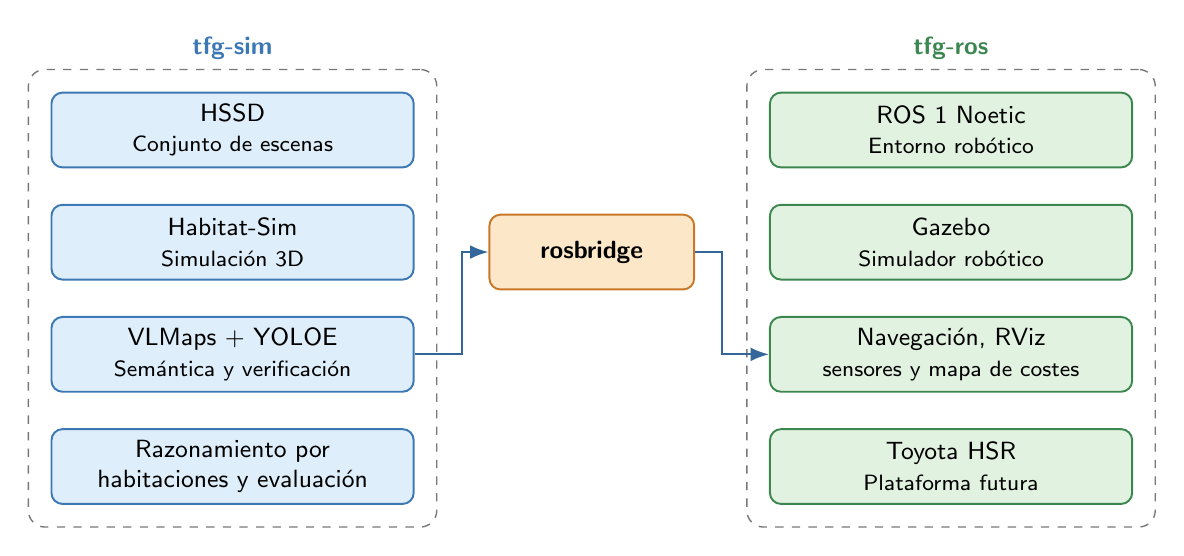
\begin{tikzpicture}[node distance=0.45cm and 0.7cm]
  \node[bloque, minimum width=4.6cm] (sim1) {HSSD\\\footnotesize Conjunto de escenas};
  \node[bloque, below=of sim1, minimum width=4.6cm] (sim2) {Habitat-Sim\\\footnotesize Simulación 3D};
  \node[bloque, below=of sim2, minimum width=4.6cm] (sim3) {VLMaps + YOLOE\\\footnotesize Semántica y verificación};
  \node[bloque, below=of sim3, minimum width=4.6cm] (sim4) {Razonamiento por\\habitaciones y evaluación};
  \node[grupo, fit=(sim1) (sim2) (sim3) (sim4), label={[anchor=south, font=\sffamily\bfseries\small, text=figAzulBorde]north:tfg-sim}] {};

  \node[bloquev, minimum width=4.6cm, right=4.5cm of sim1] (ros1) {ROS 1 Noetic\\\footnotesize Entorno robótico};
  \node[bloquev, below=of ros1, minimum width=4.6cm] (ros2) {Gazebo\\\footnotesize Simulador robótico};
  \node[bloquev, below=of ros2, minimum width=4.6cm] (ros3) {Navegación, RViz\\\footnotesize sensores y mapa de costes};
  \node[bloquev, below=of ros3, minimum width=4.6cm] (ros4) {Toyota HSR\\\footnotesize Plataforma futura};
  \node[grupo, fit=(ros1) (ros2) (ros3) (ros4), label={[anchor=south, font=\sffamily\bfseries\small, text=figVerdeBorde]north:tfg-ros}] {};

  \node[bloquen, font=\sffamily\bfseries\small] at ($(sim1.east)!0.5!(ros1.west) + (0,-1.55)$) (bridge) {rosbridge};
  \draw[flecha] (sim3.east) -- ++(0.6,0) |- (bridge.west);
  \draw[flecha] (bridge.east) -| ($(ros3.west) + (-0.6,0)$) -- (ros3.west);
\end{tikzpicture}
\caption[Arquitectura de doble contenedor.]{Doble contenedor: \texttt{tfg-sim} para la capa semántica y \texttt{tfg-ros} para la navegación robótica, comunicados con rosbridge.}
\label{fig:doble_contenedor}
\end{figure}

El objetivo a medio plazo es preparar la integración con el Toyota HSR, un robot móvil doméstico de servicio diseñado para tareas en entornos del hogar. ROS, Gazebo y RViz aportan un entorno robótico más cercano a un robot real y permiten validar la navegación con costes, mapa global, sensores láser y planificadores estándar. Dentro del periodo de prácticas la migración quedó limitada a la preparación inicial del entorno y a su validación funcional; la integración completa de la navegación y la conexión con la capa semántica se aborda ya dentro del TFG.

\paragraph{Trabajo con objetos pequeños.} Otra línea consiste en mejorar la búsqueda de objetos pequeños como botellas, tazas o portátiles. Estos objetos no aparecen de forma fiable en el mapa semántico, pero sí pueden asociarse a muebles y zonas plausibles. La estrategia adoptada es usar el mapa semántico para localizar esas zonas, YOLOE para confirmar el objeto y el razonamiento por habitaciones para acotar dónde buscar. El flujo queda documentado en la figura~\ref{fig:flujo_objetos_pequenos}; la robustez simplificada queda resumida en la figura~\ref{fig:mejora_simplificada} y sirve como base para la posterior integración con ROS.

\paragraph{Posible validación futura.} Como horizonte más amplio, una vez consolidada la migración a ROS y Gazebo, se plantea una validación más realista con el Toyota HSR simulado. Si las condiciones lo permiten, la misma división modular podría trasladarse a un entorno físico: decisión semántica en una capa y navegación robótica en otra. Estas pruebas quedan fuera del alcance de las prácticas y pertenecen al cierre del TFG.


%----------------------------------------------------------------------------------------
%	CAPÍTULO 5: RESUMEN COMPETENCIAS
%----------------------------------------------------------------------------------------

\chapter{Resumen Competencias}\label{chap:competencias}

El Grado en Inteligencia Robótica de la Universitat Jaume I, según el plan de estudios publicado en el Boletín Oficial del Estado en 2022, se organiza en torno a la programación, la electrónica, la inteligencia artificial, la visión por computador, la robótica móvil, la manipulación, el control automático y la integración de sistemas. Buena parte de las decisiones técnicas tomadas durante las prácticas se apoyan, de forma muy directa, en asignaturas concretas de ese plan. En este capítulo se vinculan ambos planos para mostrar cómo la formación previa se ha traducido en herramientas de trabajo durante la estancia, y qué nuevos conocimientos se han adquirido más allá del grado.

\section{Competencias del grado aplicadas}

En lugar de hablar de áreas genéricas, en este apartado se enlaza cada herramienta o decisión del proyecto con la asignatura concreta en la que adquirí la base que permitió afrontarla. Las asignaturas que se mencionan se corresponden con las recogidas en el plan oficial. Para facilitar la lectura, se agrupan por el curso del grado en el que se imparten.

\cursoTitulo{Primer curso}

\paragraph{Programación I, Programación II y Programación Avanzada.} Estas asignaturas me dieron la base de programación estructurada, control de flujo, manejo de estructuras de datos y diseño modular. Gracias a ello pude organizar el proyecto en piezas independientes (interpretación de la instrucción, mapa semántico, selector de habitación, navegación, verificación visual y registro), separar responsabilidades con contratos claros entre módulos y depurar cada componente por separado antes de integrarlo en el flujo completo. Toda la implementación del sistema, escrita principalmente en Python, se apoya directamente en lo aprendido aquí.

\paragraph{Laboratorio de Sistemas Operativos.} Esta asignatura me dio soltura en entornos Linux, terminal, permisos, procesos y redirección de salida. Gracias a esa base pude trabajar con contenedores Docker, configurar el entorno de ejecución, escribir guiones de arranque, automatizar tareas repetitivas y diagnosticar problemas concretos del sistema operativo cuando los componentes interactuaban entre sí.

\paragraph{Introducción a la Inteligencia Robótica.} Como asignatura introductoria del grado, me proporcionó la visión global del campo y el vocabulario común que ha sido útil al integrarme en un grupo de investigación con líneas muy diversas, donde había que entender desde la percepción semántica hasta la manipulación móvil.

\cursoTitulo{Segundo curso}

\paragraph{Sensores y Actuadores.} Me proporcionó el conocimiento sobre cómo funcionan los principales sensores que aparecen en el proyecto, sobre todo los sensores RGB-D, y cómo deben tratarse las lecturas obtenidas. Sin esa base, habría costado interpretar correctamente las imágenes de profundidad del simulador, los datos del láser o la calibración de la cámara que se utilizan más adelante en la migración robótica.

\paragraph{Programación y Simulación de Robots.} Esta asignatura me permitió entender el papel de los simuladores en el ciclo de desarrollo de un robot. Apoyándome en eso, pude poner en marcha Habitat-Sim como entorno principal de pruebas, configurar las escenas, mover el robot virtual con sensores y validar el comportamiento del sistema sin necesidad de hardware. También fue clave para empezar después con Gazebo en la fase de preparación de la migración a ROS.

\paragraph{Fundamentos de Inteligencia Artificial.} Me proporcionó la base para trabajar con representaciones simbólicas, espacios de búsqueda y heurísticas de decisión. Gracias a esa formación pude organizar la búsqueda como un problema jerárquico (habitación, mueble o zona, objeto) y plantear la priorización semántica entre objeto y habitación.

\paragraph{Introducción a Redes.} Aportó la base sobre direcciones, puertos y comunicación cliente-servidor que utilicé al configurar la comunicación entre el contenedor de simulación y el contenedor de ROS, así como al establecer el puente WebSocket que utiliza rosbridge.

\cursoTitulo{Tercer curso}

\paragraph{Sistemas Automáticos y Sistemas Automáticos Avanzados.} Me dieron el lenguaje y las herramientas para razonar en términos de máquinas de estado y políticas de decisión. Gracias a esa formación pude diseñar el estado estructurado de búsqueda por habitación y plantear el ejecutor de alto nivel como una secuencia de acciones (ir a una habitación, explorar, inspeccionar un candidato, verificar el objeto y terminar), separando claramente la deliberación de la ejecución.

\paragraph{Robótica Móvil.} Esta asignatura me dio la base sobre planificación de trayectorias, mapas y obstáculos en robótica móvil. Apoyándome en eso, pude integrar la planificación de rutas con PyVisGraph, gestionar los mapas de ocupación, controlar las colisiones, replanificar trayectorias y entender cómo encajan dentro de un mapa de costes los planificadores estándar de ROS que se utilizan en la fase de migración.

\paragraph{Visión Artificial.} Me aportó la base sobre formación de imagen, calibración de cámara, segmentación y descriptores visuales. Gracias a eso pude integrar VLMaps como representación semántica del entorno, interpretar correctamente sus mapas de calor por categoría y entender qué hace internamente un detector visual de vocabulario abierto como YOLOE en la fase de verificación.

\paragraph{Reconocimiento de Patrones y Sistemas Inteligentes.} Me proporcionaron la base para trabajar con clasificadores, espacios de características y razonamiento de alto nivel. Combinada con la formación en inteligencia artificial, esta base me ayudó a apoyarme en sugerencias del modelo de lenguaje de forma controlada y no como caja negra.

\cursoTitulo{Cuarto curso}

\paragraph{Aprendizaje Automático.} Me dio el marco para entender los modelos de visión-lenguaje (CLIP, LSeg) sobre los que se apoya VLMaps y los detectores de vocabulario abierto como YOLOE. Esta base permitió interpretar los resultados de estos modelos, reconocer sus limitaciones (por ejemplo, su debilidad ante objetos pequeños) y combinar varios modelos de forma razonada.

\section{Nuevos conocimientos adquiridos}

Más allá de las asignaturas anteriores, las prácticas me han permitido aprender técnicas y herramientas que no había trabajado en el grado. A continuación se destacan las más relevantes.

\paragraph{Mapas semánticos basados en visión-lenguaje.} El uso real de VLMaps me ha permitido entender cómo se combinan los modelos de visión-lenguaje (CLIP y LSeg) para asociar regiones del entorno con categorías generales, y cómo se proyecta esa información sobre un mapa 2D usable para navegación. Este es un ámbito mucho más reciente que el contenido habitual de las asignaturas y ha supuesto un aprendizaje importante.

\paragraph{Detección de vocabulario abierto.} La integración de YOLOE me ha enseñado el valor de los detectores que aceptan etiquetas arbitrarias y no solo un conjunto fijo, así como las precauciones que requieren al evaluar resultados (umbrales, tamaño del objeto, multiángulo).

\paragraph{Búsqueda jerárquica guiada por lenguaje.} Aprender a estructurar la búsqueda en tres niveles (habitación, mueble o zona, objeto) y a apoyarme en un modelo de lenguaje como ayuda para decidir, no como controlador, es uno de los aprendizajes más útiles del periodo.

\paragraph{Integración de sistemas complejos.} La parte más educativa del proyecto ha sido aprender a integrar herramientas heterogéneas (simulador, mapa semántico, modelo de lenguaje, detector visual) sin que ninguna ponga en riesgo la estabilidad del conjunto. Este aprendizaje incluye la depuración cuando varios componentes interactúan a la vez y la importancia de aislar fallos en un proyecto con dependencias en cascada.

\paragraph{Trabajo en un grupo de investigación internacional.} El proyecto se ha realizado en un grupo donde se discute con frecuencia y donde la documentación es parte del trabajo. He mejorado en redacción técnica clara, en planificación flexible y en presentación del avance, competencias que no se trabajan tanto durante el grado y que son determinantes en un entorno de investigación.


%----------------------------------------------------------------------------------------
%	CAPÍTULO 6: CONCLUSIÓN
%----------------------------------------------------------------------------------------

\chapter{Conclusión}\label{chap:conclusion}

La estancia en el Vision for Robotics Group de TU Wien ha permitido aplicar conocimientos del grado en un contexto de investigación real y desarrollar un proyecto que combina percepción, semántica, navegación y evaluación. Su principal valor ha sido trabajar sobre un sistema integrado, donde las decisiones técnicas solo son válidas si funcionan dentro del conjunto.

En el plano técnico, el proyecto ha pasado de una base inicial centrada en preparar el entorno a una arquitectura capaz de interpretar una instrucción en lenguaje natural, decidir dónde buscar y verificar visualmente la presencia del objeto. Esta memoria recoge únicamente el trabajo correspondiente a las 150 horas de la asignatura IR2137 y deja separada la continuidad que se desarrolla dentro del Trabajo de Final de Grado.

La aportación principal del periodo ha sido reorientar la búsqueda semántica hacia un razonamiento por habitaciones. En lugar de operar sobre un orden global del mapa, el sistema decide primero la habitación, después el mueble o zona y, por último, el objeto concreto. Esta organización jerárquica es más natural, hace la evaluación más interpretable y prepara mejor el sistema para una futura integración robótica.

A nivel de aprendizaje, la experiencia ha confirmado una idea central en robótica: la integración y la validación son tan importantes como el algoritmo. Combinar simulación, modelos de visión-lenguaje y planificación exige depurar fallos encadenados y equilibrar la calidad teórica de cada componente con la robustez del sistema completo. He aprendido a planificar de forma flexible y a consolidar la base antes de añadir nuevas capacidades.

En el plano personal, la estancia en Viena también ha sido una experiencia formativa importante. Trabajar en un país distinto, dentro de un grupo internacional y en un idioma de trabajo no nativo me ha obligado a comunicarme con precisión, adaptar mi forma de organizar el trabajo y defender decisiones técnicas con claridad.

Por último, las prácticas han reforzado mi motivación por continuar trabajando en percepción, semántica y navegación robótica. El proyecto queda preparado para profundizar en el TFG mediante evaluación cuantitativa, migración a ROS y Gazebo y, eventualmente, integración con el Toyota HSR. Esta continuidad cierra de forma natural el periodo de prácticas y abre una nueva fase del trabajo.


%----------------------------------------------------------------------------------------
%	BIBLIOGRAFÍA
%----------------------------------------------------------------------------------------

\chapter{Bibliografía}

A continuación se presentan las referencias citadas a lo largo de la memoria. Incluyen las publicaciones en las que se basan los principales componentes del sistema (modelos de visión-lenguaje, detectores de vocabulario abierto, simuladores y conjuntos de escenas) y las herramientas de soporte utilizadas durante la estancia.

\nocite{huang2023vlmaps}
\nocite{chang2017matterport3d}
\nocite{wang2025yoloe}
\nocite{radford2021clip}
\nocite{li2022lseg}
\nocite{savva2019habitat}
\nocite{szot2021habitat2}
\nocite{khanna2024hssd}
\nocite{honerkamp2024moma}
\nocite{quigley2009ros}
\nocite{koenig2004gazebo}
\nocite{yamamoto2019hsr}
\nocite{crick2017rosbridge}
\nocite{wada2016labelme}
\nocite{docker2013}
\nocite{nvidia2007cuda}

\printbibliography[heading=bibempty]

%----------------------------------------------------------------------------------------

\end{document}
